% overview.tex
% RICHARD NOTE:
%   Original version:
%      Planning/ShortProjectEvaluations/2013-08-MeBradyEtAl-MarginalizedPE/overview.tex
\documentclass[twocolumn,prd,nofootinbib]{revtex4}
%\newcommand\ForRichardOnly[1]{#1}
\newcommand\ForRichardOnly[1]{}
\usepackage{verbatim}
\usepackage{color}     % color text
\usepackage{framed}
\definecolor{shadecolor}{gray}{0.95}
\usepackage{amsmath}
\usepackage{graphicx}  % extend graphics
\usepackage{tabularx}
\usepackage{wrapfig}   % wrap text around figures, if desired
\usepackage{hyperref}

% Standard LAL, LALAPPs links
\newcommand\LALDocsMain{\href{http://www.lsc-group.phys.uwm.edu/lal/slug/nightly/doc/lsd-nightly.pdf}{LALDocs}}
%\newcommand\LALappsDocsMain{\href{http://www.lsc-group.phys.uwm.edu/~saikat/doc/lalapps.pdf}{LALapps docs}}
\newcommand\LALappsDocsMain{\href{http://www.lsc-group.phys.uwm.edu/lal/slug/nightly/doc/lalapps-nightly.pdf}{LALapps docs}}
\newcommand\LALDocsSource[1]{\href{http://www.lsc-group.phys.uwm.edu/cgit/lalsuite/tree/#1}{#1}}
\newcommand\LALDocsSourceInline[2]{\href{http://www.lsc-group.phys.uwm.edu/cgit/lalsuite/tree/#1}{{\tt #2}}}

% BONUS TOOLS

\newcommand\editremark[1]{{\color{red} #1}}

\newcommand\unit[1]{\, {\rm #1}}
\newcommand\aap{A\&A}
\newcommand\apss{APSS}
\newcommand\aaps{AAPS}
\newcommand\apjs{ApJ S}
\newcommand\aj{AJ}
\newcommand\apjl{ApJL}
\newcommand\mnras{MNRAS}
\newcommand\pasp{PASP}
\newcommand\araa{ARA\&A}
\newcommand\physrep{Phys. Rep.}
\newcommand\aapr{AAPR}
\newcommand\nar{NAR}  % New astronomy reviews

\newcommand\sigmahat{\hat{\sigma}}
\DeclareMathOperator{\sgn}{sgn}
\DeclareMathOperator{\erf}{erf}

\newcommand\Y[1]{Y^{(#1)}{}}
% GR tools
\newcommand\prederiv[2]{{}^{(#1)}#2}
\newcommand\dualBack{*}
\newcommand\dualForward{\star}
\newcommand\avL{\left< {\cal L}_{(a} {\cal L}_{b)} \right>}
\newcommand\WeylScalar{{\psi_4}}
\newcommand\WeylScalarFourier{{\tilde{\psi}_4}}
\newcommand\mc{{{\cal M}_c}}
% QM TOOLS
\newcommand\qmstate[1]{\left|#1\right \rangle}
\newcommand\qmstateKet[1]{\left\langle#1\right|}
\newcommand\qmstateproduct[2]{\left\langle#1|#2\right\rangle}
\newcommand\qmoperatorelement[3]{\left\langle#1\left|#2\right|#3\right\rangle}
\newcommand\qmoperator[1]{{\bf #1}}


\begin{document}

\title{PE by Monte Carlo}
\author{R. O'Shaughnessy}
\author{E. Ochsner}
\author{C. Pankow}
\author{P. Brady}
\author{H. Qi}
\begin{abstract}
Notes. Main content in white.  Gray sidebars are ``footnotes'': implementation tricks and comments to be skipped on a
first read.
\end{abstract}
\maketitle
\tableofcontents
\part{Notes for group}
\nocite{gwastro-HarryFairhurst-CoherentTargetedSearch}
% Keppel http://adsabs.harvard.edu/cgi-bin/nph-data_query?bibcode=2012arXiv1208.2340K&link_type=ABSTRACT


\begin{widetext}

\noindent \textbf{Action items}

\begin{verbatim}
- Richard:
  - Convergence rate theory for sampler
  - Sky sampler check
  - Bughunt
- Evan : 
  - dag layout  (perhaps stochastic banks? perhaps tmptbank + jitter)
     Harvest from pycbc if needed

- Chris

 - modified sampler: sky location done directly (via explicit loop)


Feedback for Chris
  - neff has a fencepost error

\end{verbatim}
\end{widetext}

%% Long term
%%   - dag 
%%   - priming future with past: Each MC evaluation provides information about intrinsic parameters, which we can use to further refine subsequent iterations.  Convergence should get faster as we go.

%%   - filtering to allow us to work with downsampled data (if viable).
%%     May be tricky because of timing and sky location issues.

%%   - psd issues and high frequency: will truncating the PSD at say 2048 due to sampling 
%%     contaminate our recovered parameters if time resolution (i.e., SNR) ought to be  very high?


\section{What we are selling}

\subsection{Early sale}

\noindent \textbf{Showing off}:
\begin{itemize}
\item \emph{Viable for expensive waveforms} Our approach is not limited by waveform generation costs.  We can therefore perform
robust parameter estimation with ``expensive'' waveforms like SEOBNR and EOBNRv2HM.  And we have [provide examples]

\item \emph{Viable for expensive long data}: Our approach is not limited by ``setup'' cost and works well with \emph{long} data
  stretches, such as signals with many resolved higher harmonics; BNS in aLIGO; etc.

\item \emph{Reliable evidence}: The evidence is the principal figure of merit for parameter estimation,
particularly for selecting among models of competing sophistication.   

Our code provides an  reliable evidence calculation, with well-understood error bars.
\end{itemize}


\noindent \textbf{Playing to the crowd}: At the Sept LVC in Hannover, the PE group identified waveform systematics as a
core issue needing futher development.  To address waveform systematics (i.e., varying PN order; modified GR) as well as
technically useful approximations (i.e., the inclusion of higher harmonics; the low-frequency cutoff when doing so) we
need a much faster code, better-suited to large-scale simulations in gaussian noise. 

Our code meets this gap, providing a fast and theoretically-easily-understood procedure to compare waveform families in
gaussian noise.  

\emph{In addition}, this fast procedure may provide ultra-low-latency parameter estimation.

\section{Stage 0: What are we calculating}

\subsection{The reduced likelihood}
\noindent \textbf{Gravitational wave signal}: Paramters $\lambda,\theta$ for $\lambda$ intrinsic parameters (slow) and
$\theta$ extrinsic parameters (fast).  The code provides $h(t|\lambda,\theta)$ in the Earth's geocenter or, more
usefeul, $h_{lm}$, a spin-weighted spherical harmonic decomposition relative to the emission direction $\hat{N}$
\begin{shaded}
\begin{itemize}
\item $h(t)=h_+-i h_\times$ is a complex strain unless explicitly indicated otherwise.   Capital letters $H$ denote
  quantities in a particular detector's data stream.  The hatted quantity $\hat{H}_k$ is the measured strain data in the
  $k$th detector.
\item All operations respect polarization symmetry and time translation.  Under a rotation by $\psi$ around the
  propagation direction, the waveform transforms as
\[
h' = h \exp(-2i \psi)
\]
\item The source propagation direction away from the source is $\hat{n}(\theta_{JN},\phi_{JN})$ where
  $\theta_{JN},\phi_{JN}$ are the angles of the propagation direction relative to the total angular momentum vector (at
  some time) $J$; the projection of $J$
  onto the plane of the sky is $\psi_J$.  The spin-weighted
  spherical harmonic decomposition is 
\begin{eqnarray}
\label{eq:def:hSpinWeightEmissionDirection}
h(t|\lambda,\theta) = \sum_{lm} h_{lm}(t|\lambda) e^{-2i\psi_J}\Y{-2}_{lm}(\theta_{JN}\phi_{JN})
\end{eqnarray}
Note $h_{lm}$ depends only on intrinsic parameters.  (Implicitly, $h_{lm}$ also depends on our choice of reference
frequency, typically 100 Hz.).  Coefficient functions $h_{lm}$ are provided in
\cite{gw-astro-mergers-approximations-SpinningPNHigherHarmonics}; the theory underlying orbital phase generation is
summarized in  \cite{gw-astro-PN-Comparison-AlessandraSathya2009}, etc.
\item The sky location is $\hat{n}=\hat{n}(\delta,\alpha)$ (i.e., RA and DEC angles).  we do not have to do sky location
  conversions ourselves.
\item Fourier sign convention is as follows, consistent with \cite{gwastro-mergers-nr-Alignment-ROS-Polarization}
\begin{eqnarray}
h(t) = \int \frac{d \omega}{2\pi} \; e^{-i\omega t} \tilde{h}(\omega) \\
\tilde{h}(2\pi f) = \int dt e^{i 2\pi f t} h(t)
\end{eqnarray}
In the common case that  $h = Ae^{-i\Phi(t)}$ with $\Phi$ increasing monotonically, the fourier transform $\tilde{h}(f)$ will be dominated by
positive-frequency components
\end{itemize}
In practice $h(t)$ is timesampled at some fixed rate for its entire duration.  The signal duration is dominated by
low-frequency content.
\end{shaded}


\noindent \textbf{Response of each detector}: Each detector has a response function which returns some $H_k(t)$, the
``strain'' function of that detector.  No matter how complicated the response, it must satisfy time-translation symmetry and spin-weight-$-2$ symmetry.
 \emph{Generic} detector response must account for arbitrary frequency
content at each time and requires slow calculations to carefully propagate signals with $f\simeq f_{FSR}$.  

In the
\emph{long wavelength limit} the response can be approximated using some $F_+,F_\times(t)$:
\begin{align}
H_k(t) &=F_{+,k}(t) h_+(t-\vec{x}_k(t)\cdot \hat{k}) + F_\times(t) h_\times(t-\vec{x}_k(t)\cdot \hat{k}) \\
 &= \text{Re}(F_++i F_\times)_k h(t-\vec{x}_k(t)\cdot \hat{k}) \\
 &=  \frac{F h }{2} + \frac{F^*h^*}{2} \equiv (Fh  + F^*{\cal I} h)/2
\end{align}
where $-\hat{k}$ points toward the sky location, \emph{opposite} to the direction of propagation $\hat{k}$; where $F=F_++i F_\times$;
where $F_{+,\times}$ are calculated as $F_+(t)=e_+^{ab}d_{ab}(t)/2$ and follow by contracting a unit tensor with the time-dependent geometry tensor of each
interferometer; where self-evident dependence on $t$ and $t-\hat{k}\cdot \vec{x}_k$ has been suppressed; and
where ${\cal I}$ is the (complex-antilinear!) complex conjugation operation in time.   
\begin{shaded}
\noindent \textbf{A ``complex conjugate''}: What is  ${\cal I}$? I want to take fourier transforms of the complex
conjugate of a  complex function of time
unambiguously.  So ${\cal I}$ is the ``complex conjugate in time'' operation:
\begin{align}
{\cal I}\tilde{h}(\omega) &\equiv \int e^{-i\omega t} h(t)^* dt  = [\tilde{h}(-\omega)]^* \\
{\cal I} p h &= p^* {\cal I} h \\
(a,{\cal I} b) & = (b,{\cal I}a) = 2 \int_{-\infty}^{\infty} df \frac{[\tilde{a}(f)]^*[\tilde{b}(-f)]^*}{S_h(|f|)}\\
 &= ({\cal I} a,b)^*
\end{align}
which trivially satisfies ${\cal I}^2=1$.  Remember ${\cal I}$ is \emph{not} linear, as ${\cal I} i h = -i {\cal I} h$
and hence ${\cal I}F=F^*{\cal I}$.  
Because of how it prefers time, however, it will \emph{not} conjugate  $i\omega$ (i.e., time translations):  if $h'(t)=h(t-\Delta t)$, then 
\begin{eqnarray}
\tilde{h}' = e^{-i\omega \Delta t}\tilde{h} \qquad {\cal I}\tilde{h}' = e^{-i\omega \Delta t} {\cal I}\tilde{h}
\end{eqnarray}


\noindent \textbf{Complex inner products}: I want to use a hilbert space, allowing complex arguments.  My preferred inner product is
therefore complex-valued; see \cite{gwastro-mergers-HeeSuk-FisherMatrixWithAmplitudeCorrections}. 
\end{shaded}

\begin{shaded}
\noindent \textbf{Evaluating the response functions}
The beampattern operations $F_{+,\times}$ are applied in the time domain. The translation to each detector position is
applied using a set of short fourier transforms.  The cost to construct $H_k$ from $h$ is therefore  $\simeq N_{samp}\ln
N_{samp}$ for $N_{samp} = \ln
T/\Delta t$.

For a sufficiently short-duration source, both the beampattern functions and detector positions can be approximated by
constants.  Strictly, this limit does not hold for binary neutron stars.  As a first approximation, however, we can
probably assume  the fourier transform $\tilde{H}_k[h]$ can be re-expressed as 
\begin{eqnarray}
\tilde{H}_k = \frac{e^{i\omega \hat{k}\cdot \vec{x}_k}}{2}\left[ 
   F_k  \tilde{h} + F_k^* {\cal I} \tilde{h} 
 \right]
\end{eqnarray}
[Physically, equation reflects a common time translation applied to two basis signals appearing in  $\text{Re} F h$.]
\end{shaded}


\noindent \textbf{Likelihood}: Each detector has a noise power spectrum $S_{h,k}$, assumed known and
stationary, defining an inner product $\qmstateproduct{a}{b}_k \equiv 2 \int_{-\infty}^\infty  a^*(f)b(f)/S_{h,k}(f)$ on
complex-valued functions $a,b$ of time.  Each detector has strain data $\hat{H}_k(t)$.  We evaluate the following likelihood ratio for each element
\begin{eqnarray}
-2\ln L_k &= \qmstateproduct{H_k-\hat{H}_k}{H_k-\hat{H}_k}_k - \qmstateproduct{\hat{H}_k}{\hat{H}_k}_k \\
  &= \qmstateproduct{H_k}{H_k}_k - 2 \text{Re} \qmstateproduct{H_k}{\hat{H}_k}_k 
\end{eqnarray}
The total likelihood is the product of individual detectors' likelihoods:
\begin{eqnarray}
\ln L &\equiv \sum_k \ln L_k  = \ln L_{\rm model} + \ln L_{\rm data} \\
\ln L_{\rm model} &\equiv -\frac{1}{2} \sum_k \qmstateproduct{H_k}{H_k}_k \equiv - \rho^2/2 \\
\ln L_{\rm data} &\equiv  \sum_k \qmstateproduct{H_k}{\hat{H}_k}_k 
\end{eqnarray}
\ForRichardOnly{
\begin{shaded}
\textbf{Efficiency of terms?}: As described below, the two terms in the log likelihood
\begin{itemize}
\item \emph{Model-only term}: This time-translation-independent $L_{\rm model}$ can be efficienly calculated from $\tilde{h}$ in the
  geocenter, for any sky location [Eq. \editremark{X}], from an O(N) operation.  To get $\tilde{h}$ in the geocenter for
  an arbitrary \emph{emission} direction, we need to sum over $\tilde{h}_{lm}(f)$ via
  Eq. (\ref{eq:def:hSpinWeightEmissionDirection})
\item \emph{Data term}: The other term can be efficiently computed for all times, sky locations, and emission directions
  by archiving $\qmstateproduct{h_{lm}\exp(-i\omega t)}{\hat{H}_k}$ timeseries [Eq. (\ref{eq:IndividualDetectorLikelihoodTimeseries:ViaSpinWeightBasis})].
\end{itemize}
\end{shaded}
}

\begin{widetext}
\begin{shaded}
\noindent \textbf{Reorganize?}
Using the notation in  \citet{gwastro-mergers-HeeSuk-CompareToPE-Aligned}, we define 
\begin{eqnarray}
-2 \ln L &\equiv \rho^2 - 2 \sum_k \qmstateproduct{H_k}{\hat{H}_k}
\end{eqnarray}
The first term is time-translation invariant and ``easy'' to evaluate ``once and for all'' -- see later tricks with
$h_{lm}$.   The second term can be resummed by substituting the value of $H_k$ in terms of translations, beampatterns,
and $h(t)$ at the geocenter.  So...


\noindent \textbf{Coherent likelihood for a stationary network}: Assume $\vec{x}_k$ and $F_k$ are  stationary, so
$\tilde{H}_k(f)$ is easily evaluated and substituted: 
%\editremark{fix definitions: be consistent with old notation; make sure I include both terms}
\begin{align}
\label{eq:def:GeocenteredInnerProductWithData}
\sum_k \qmstateproduct{H_k}{\hat{H}_k}_k 
& = 
 \sum_k \frac{1}{2}\left [ \qmstateproduct{ F_k h +  F_k^*{\cal I}h}{e^{i\omega \hat{k}\cdot \hat{x}_k} \hat{H}_k}_k
 \right]
= \text{Re} \qmstateproduct{h}{{\cal S}}_{\rm ref} \\
\tilde{{\cal S}}(f) &= \sum_k \hat{H}_k(f) \frac{S_{\rm ref}}{S_{k}} F_k^* e^{-i\omega \hat{k}\cdot \vec{x}_k} \equiv \sum_k {\cal S}_k\\
{\cal S}(t) &= \sum_k F_k^* H_k(t+\vec{x}_k\cdot \hat{k}) \quad \text{if all detectors identical}
\end{align}
The inner product $\qmstateproduct{.}{.}_{\rm ref}$ uses a reference PSD; exact equality holds for any choice, including
a geometric mean PSD or a single reference interferometer:
\begin{eqnarray}
S_{\rm ref}^{-1} = \frac{1}{N_{\rm det}} \sum_k S_{k}(f)^{-1} \quad ;\text{or} \quad  S_{\rm ref} = S_1
\end{eqnarray}
%
In this form, the translated detector data carries all information about the sky location; no information about the
source is used.  The data from each detector is \emph{geocentered} by first applying the \emph{inverse} time
translation operation; then the beampattern response and detector PSD, as a weight.
%

Similarly, the signal amplitude can be expressed using geocentered quantities.  Taking care to allow for different PSDs
in different detectors, we find
\begin{align}
\label{eq:CalculateRhoFromGeocenterStrain}
\rho^2& \equiv \sum_k \qmstateproduct{H_k}{H_k}_k 
 =  \frac{1}{2}\qmoperatorelement{h}{\sum_k F_k^* F_k\frac{S_{\rm ref}}{S_k}}{h}_{\rm ref} 
 + \frac{1}{4}\qmoperatorelement{h}{\sum_k F_k^* F_k^* \frac{S_{\rm ref}}{S_k}}{{\cal I} h}_{\rm ref}  
 + \frac{1}{4}\qmoperatorelement{{\cal     I}h}{\sum_k F_k F_k \frac{S_{\rm ref}}{S_k}}{h}_{\rm ref}  \\
&\equiv  \qmoperatorelement{h}{\sigma}{h}_{\rm ref}  + \frac{\text{Re}}{2} \qmoperatorelement{h}{\zeta^*}{{\cal I}
   h}_{\rm ref}
\end{align}
where the last expression implicitly defines the operators $\sigma(f|\hat{k}), \zeta(f|\hat{k})$:
\begin{eqnarray}
\sigma \equiv \frac{1}{2} \sum_k |F_k|^2 \frac{S_{\rm ref}(f)}{S_k(f)} 
\qquad 
\zeta \equiv \sum_k F_k F_k \frac{S_{\rm ref}(f)}{S_k(f)} 
\end{eqnarray}

\noindent \textbf{Why do we care, mark 1}: This operation [Eq. (\ref{eq:def:GeocenteredInnerProductWithData})] allows us to quickly explore any individual sky location.  And to
explore alternative sky locations (via all possible time translations of the raw data): just reconstruct ${\cal S}$ from
the raw data streams slightly differently.   And to reduce the number of FFTs we need to perform for time translation:
having constructed ${\cal S}$, it needs to be fourier transformed only once to make the network SNR timeseries.

\noindent \textbf{Why do we care, mark 2}: Suppose we tabulate $\tilde{h}_{lm}(f)$. We can efficiently generate
$\tilde{h}$ for any emission direction [Eq. (\ref{eq:def:hSpinWeightEmissionDirection})] via an order N operation
($\tilde{h}$ depends only on emission direction, not sky position),
then efficiently generate $\rho^2$ for any sky location via an O(N) operation [the inner product with these
  sky-position-dependent operations].  

To be even more efficient, we can pre-tabulate the $\qmstateproduct{h_{lm}}{h_{l'm'}}$, which depend only on $\lambda$
and the $k$th detector PSD, and reconstruct $\rho^2$ algebraically:
\begin{subequations}
\label{eq:ComputeRhoViaInnerProductMatrix}
\begin{align}
{\color{blue} U_{k,lm,l'm'}(\lambda)}& = \qmstateproduct{h_{lm}}{h_{l'm'}}_k \\
V_{k,lm,l'm'}(\lambda)& = \qmstateproduct{{\cal I}h_{lm}}{h_{l'm'}}_k \\
\ln L_{\rm model}(\lambda|\hat{n},\hat{k},\psi_J,d) &=
   -\frac{(d_{\rm ref}/d)^2}{2}\sum_k
\left[
{\color{blue}
 \frac{1}{2}|F_k(-\hat{k})|^2 U_{k,lm,lm'}(\lambda)[\Y{-2}_{lm}(\hat{n})]^*\Y{-2}_{l'm'}(\hat{n})
}
 \right. \nonumber \\ & \left.
 {\color{blue}
+
 \frac{1}{2} \text{Re} V_{k,lm,l'm'} e^{-4i\psi_J}F_k^2 \Y{-2}_{lm}(\hat{n})\Y{-2}_{l'm'}(\hat{n})
}
\right]
\end{align}
\end{subequations}

\noindent \emph{Implementation tricks}: To minmize confusion, I recommend evaluating ${\cal I}h_{lm}(t)$ in the time
domain and fourier transforming it, so it has exactly the same code path as $\tilde{h}_{lm}(f)$; for speed you can use
${\cal I}\tilde{h}_{lm}(f) = h_{lm}(-f)^*$ if you are careful.

For nonprecessing binaries $\tilde{h}_{lm}(-f)^*=(-1)^lh_{l,-m}$ and therefore $V_{k,lm,l'm'} = (-1)^l U_{k,l-m,l'm'}$
\end{shaded}

\end{widetext}




\noindent \textbf{Reduced likelihood}: The reduced likelihood combines all detectors and integrates over all prior
volume:
\begin{eqnarray}
{\color{blue} L_{\rm red} = \int p(\theta) d\theta \prod_k L_k = \int p_s(\theta) d\theta \frac{p}{p_s}\prod_k L_k }
\end{eqnarray}
where $p_s$ is our sampling prior.  Specifically, if $d_{\rm max}$ is the maximum distance allowed and $T_{window}$ the
time window, the reduced integral has the form (for \textbf{Euclidean cosmology})
\begin{eqnarray}
L_{\rm red} = \int \frac{dt}{T_{\rm window}} \frac{d^2 dd d\Omega_{sky} }{V_{\rm max}} \frac{d\Omega_{\rm
    emit}}{4\pi} \frac{d\psi}{\pi} L
\end{eqnarray}



\ForRichardOnly{
\subsection{Stage 0: Marginalize in time}
\noindent \textbf{Rationale}: For long (BNS) signals, constructing the waveform for a fixed propagation direction is expensive, because of the cost of time translation to
each site.  Let's get the most out of each sky location


\noindent \textbf{Method: FFT translation?}: The fourier transform of the inner product provides automatic time
translation on a discrete timesample grid $t_p = t_o + n\Delta t$, using a discrete FFT approximation to
\begin{align}
-2 \ln L_k(t_p)& = \qmstateproduct{H_k}{H_k}_k + 4\text{Re}\int_{-\infty}^\infty df 
  \frac{e^{-i2\pi f t_p}\tilde{H}_k(f)\tilde{\hat{H}}_k(f)}{S_{h,k}(f)} \\
-2 \ln L(t_p) & = \rho^2 -4 \text{Re}\int_{-\infty}^{\infty} df e^{-i2\pi f t_p} \sum_k\frac{\tilde{H}_k(f)\tilde{\hat{H}}_k(f)}{S_{h,k}(f)} \\
&\equiv \rho^2 - 2 \rho \hat{\rho}(t)
\end{align}
where the first term  $\qmstateproduct{H_k}{H_k}_k$ must be independent of time and where the second term defines
$\hat{\rho}(t)$, a function of time, the data, and the template.   Marginalization over event time therefore corresponds to using these sample points to evaluate
the integral:
\begin{eqnarray}
\int dt L p_t(t)  = \frac{1}{T_{window}} \int_{t_{start}}^{t_{start}+T_{window}}dt  e^{\ln L}
\end{eqnarray}

\begin{shaded}
\noindent \textbf{Quadrature}: A typical low sample rate (few kHz) is often not enough to
evaluate the integrand in the likelihood with a naive (box) quadrature.  Very high sampling rates \textbf{or interpolating the
  integrand $L_k$  and integrading accordingly}  are needed to integrate the likelihood.

We can use any intelligent quadrature method we want for the integral -- including locally interpolating the integrand
$L$ to make a locally continuous function and integrating with any quadrature desired. 

%For speed, we may want a \emph{rejection approximation}: approximate the integrand as \emph{zero} if the max log
%likelihood is less than a certain value, or the posterior is distributed widely in time.  (Not clear if this saves us
%much: we have already done the FFT.)

\noindent \textbf{${\cal S}$ and coherent data}:  If organized intelligently, only one inverse FFT is needed to
construct $\hat{\rho}(t)$ for each sky location.  [An even better scheme uses only one inverse FFT per detector for
  \emph{all} sky locations...see $h_{lm}$ later.]

%% \noindent \textbf{Massively less than unity?}: For a physical source,  the log likelihood will be massively less than
%% unity almost everywhere.   If we just want reliable parameter estimates
\end{shaded}


\subsection{Stage 1: Marginalize in time and polarization angle}

\noindent \textbf{Rationale}: As above.
%
In GW searches, time and polarization phase marginalization is done simultaneously.  At each timesample, we expected we could
 marginalize \emph{analytically} over polarization phase, with a bessel function.

That's not true.

\noindent \textbf{Challenges}: In general the detector network and source (aka data) have preferred orientations.  These
orientations need not agree.  
\begin{shaded}
\noindent \textbf{Template amplitude}: Using the $\sigma,\epsilon$ notation of \citet{CutlerFlanagan:1994}, the signal amplitude term has the form $\rho^2 = \sigma
\rho_0^2(1+\epsilon \cos 4(\psi-\psi_0))$ where $\rho_0^2$ is the amplitude of a source directly overhead a single
detector and $\sigma,\epsilon$ are derived from the beampattern functions:
\begin{eqnarray}
C_{\lambda \lambda'}&=& \sum_k \begin{bmatrix}
F_+^2 & F_+F_\times \\
F_\times F_+ & F_\times^2
\end{bmatrix}\\
&=& \sum_k [P_k : \hat{e}_\lambda(\hat{n})] [P_k : \hat{e}_{\lambda'}(\hat{n})]  \nonumber \\
& =& \sigma U\begin{bmatrix} (1+\epsilon) & 0 \\ 0 & 1-\epsilon \end{bmatrix} U^{-1} 
\end{eqnarray}
where $U$ is a unitary transformation that diagonalizes $C$.

\noindent \textbf{Response against data}: By contrast, for a fixed data set, the second term in the likelihood
necessarily transforms like $h$: purely sinusoidally in polarization angle
\begin{eqnarray}
\rho \hat{\rho} = A \cos 2\psi + B \cos 2 \psi
\end{eqnarray}
\noindent \textbf{Marginalizing?}: If this were the only term in the likelihood -- for example, for an isotropic network
--  we could marginalize exactly: \textbf{BUT THIS IS NOT TRUE}
\begin{align}
\ln L  &= [\ln L]_c \cos 2\psi + [\ln L]_s \sin 2\psi = \ln L_0 \cos 2(\psi-\psi_0)  \\
\ln L_0 &= \sqrt{[\ln L]_c^2+[\ln L]_c^2} \\
\int_0^{\pi}\frac{ d\psi}{\pi} L &= \frac{1}{\pi}I_0(\ln L_0)
\end{align}
In general $\rho$ depends on $\psi$, so we can't: both $\cos 2\phi$ and $\cos 4\psi$ appear in the exponential, unless
the network has $\epsilon=0$ (i.e., equal sensitivity to both polarizations).
\end{shaded}



\noindent \textbf{Method: Phase alone}: We know how to evaluate all the terms in the likelihood given 4 quadrature
points at $0,\pi/4, \pi/8, 3\pi/8$.  We could hardcode the integral
\begin{eqnarray}
\int_0^{\pi}\frac{ d\psi}{\pi} e^{\ln L}
\end{eqnarray}
using values at these 4 points.   Or otherwise provide a fast way to evaluate the 1d integral, given the known form of
$\rho$ and $\qmstateproduct{h}{{\cal S}}$ veruss $\psi$

\noindent \textbf{Method: Phase and time integral}: Marginalizing over phase can be performed at each $t_p$ using the
archived values  $L(t_p, \psi)$ computed by fourier transforming the signal for several $\psi$...or by other methods.
\begin{eqnarray}
\int \frac{dt}{T_{\rm win}} \int \frac{\psi}{\pi}L
\end{eqnarray}




\subsection{Stage 2: Marginalize in time, polarization angle, and distance }

\noindent \textbf{Rationale}: As above.

\noindent \textbf{Challenges}: No analytic simplifications possible here or henceforth 

\noindent \textbf{Principle}: In each $\ln L_k$  are terms that scale quadratically with $1/d$
($\qmstateproduct{H}{H}$) and terms that scale linearly with $1/d$ ($\qmstateproduct{H}{\hat{H}}$).  If we pick one
reference value, we can rescale all terms in $L$ analytically:
\begin{align}
-2 \ln L &= \rho_{\rm ref}^2 (d_{ref}/r)^2  - 2 (d_{\rm ref}/r) \hat{\rho}\rho_{\rm ref} \\
\int L &=  \frac{dt}{T_{\rm window}} \frac{d\psi}{\pi}\int_0^{r_{rm max}} \frac{r^2 dr}{d_{\rm max}^3/3} e^{\ln L}
\end{align}
Note $\rho_{\rm ref}$ will be independent of $t$ but will depend on $\psi$, while $\hat{\rho}$

\noindent \textbf{Implementation: Generic quadrature}: All elements of the quadrature can be evaluated analytically,
from the real and imaginary parts of the fourier-transformed $\qmstateproduct{h}{{\cal S}}$.  So use something accurate
and fast -- e.g., a Monte Carlo integral with some broad distribution. 


\begin{shaded}
\noindent \textbf{Compare to  Bayestar}: Larry and Leo do a 1d distance integration with GSL : \texttt{gsl integration qagp}
\end{shaded}

}

\subsection{Stage 3: Marginalize in time, phase, distance, and emission direction  }

\noindent \textbf{Rationale}: Waveform generation and FFTs are expensive; large data sequences involve many $O(N)$
operations.   For long (BNS) signals, constructing and handling the 30 min of data is very expensive!  Let's get the most out of each sky location.

\noindent \textbf{Principle}: Express $h(t)$ and $h(f)$ using basis functions:
\begin{eqnarray}
h(t|\lambda,\theta)=\sum_{lm}h_{lm}(t)\Y{-2}_{lm}(\theta_{NJ},\phi_{NJ}) \\
h(f|\lambda,\theta)=\sum_{lm}\tilde{h}_{lm}(f)\Y{-2}_{lm}(\theta_{NJ},\phi_{NJ})
\end{eqnarray}
This identifies natural but \textbf{not   generally orthogonal} basis functions $h_{lm}$.\footnote{Particularly with higher
  harmonics and spin, orthogonality should not be assumed.}  

\noindent \textbf{Is this worth writing out?}: If we have code to generate $h(t)$ and $h(f)$ from $h_{lm}(t)$ and
$h_{lm}(f)$, do we gain anything by writing out these expansions in full?  Just have your code provide a fast cached way
to compute $h(t)$ and $h_{lm}(f)$ so we can efficiently evaluate $\rho^2$ and $\qmstateproduct{h}{{\cal S}}$?

\noindent \textbf{What could be our advantage?}: To push extreme performance, it's \emph{possible} to generate complex-valued
timeseries via the inner product of $H_k(t)$ with $h_{lm}(t-\tau)$:
\begin{eqnarray}
{\color{blue}Q_{k,lm}(\tau) \equiv \qmstateproduct{\exp(-i\omega \tau) h_{lm}}{\hat{H}_k}_k} \\
{\color{blue}P_{k,lm}(\tau) \equiv \qmstateproduct{\exp(-i\omega \tau){\cal I}h_{lm}}{\hat{H}_k}_k}\nonumber \\
 = Q_{k,lm}(\tau)^*
\end{eqnarray}
The latter equality follows either by using the definition of ${\cal I}$; by thinking of the expression as two real
inner products involving time translated $\text{Re}h_{lm}$ and $\text{Im}h_{lm}$; et cetera. 
These quantities, evaluated once and for all at each detector, can be  timeshifted to cover all sky positions as well as all orientations.  \textbf{After the
initial signal generation, fourier, comparison against data and inverse FFT, no further fourier transforms are performed. }
%
If fourier transforms dominate our computational cost, this postprocessing-only approach will be much faster.

\begin{widetext}
\noindent \emph{Longhand Implementation}: Explicit non-geocentered expressions allowing for timeshifts or sky position
shifts have the form \editremark{missing polarization angle explicitly in this construct}
\begin{align}
\label{eq:IndividualDetectorLikelihoodTimeseries:ViaSpinWeightBasis}
\sum_k\qmstateproduct{e^{-i \omega \tau} H_k}{\hat{H}_k}_k
&= \frac{1}{2} \sum_k (F_k \Y{-2}_{lm})^* {\color{blue} \qmstateproduct{ h_{lm}}{e^{i\omega t}\hat{H}_k}_k}
   + (F_k \Y{-2}_{lm}) {\color{blue}\qmstateproduct{{\cal I} h_{lm}}{e^{i\omega t}\hat{H}_k}_k} \\
 &= \sum_k \text{Re}[(F_k(-\hat{k}) \Y{-2}_{lm}(\hat{n}))^* Q_{k,km}(\tau|\lambda)]
\end{align}
The blue expressions have the form $\qmstateproduct{h_{lm}}{\hat{H}_k}_k$.  For a nonprecessing source ${\cal I} h_{lm}
=(-1)^l h_{l,-m}$, letting us reduce by $\times 2$ the number of inverse FFTs needed; in general no symmetry holds. 

\end{widetext}

\begin{shaded}
\noindent \textbf{Basis signals?}: Several methods exist to identify natural basis signals in
$h$.  For generic sources, some polarization angle $\psi$ exists such that for $h'\equiv h \exp(-2i\psi)$,
$h_+'$ and  $h'_\times$ are  orthogonal\footnote{%
The matrix $B_{ss'} =\qmstateproduct{h_s}{h_{s'}}$ with $s=+,\times$ is a positive-definite symmetric matrix.  Rotating
to its eigenbasis proves the claim and identifies the polarization angle needed.}
For generic sources,  the positive- and negative-frequency parts of $h$ are also trivially orthogonal and  correspond to left- and
right-handed radiation.\footnote{ in simple cases,  these two parts may be proportional to complex-conjugates of one
another but that breaks down in general.  }
In general we don't have ``cosine'' and ``sine'' chirps, particularly with higher harmonics and spin.

This situation should be contrasted with the assumptions implicit in the F statistic
\cite{gwastro-HarryFairhurst-CoherentTargetedSearch}, which de facto makes the cosine/sine chirp assumption; BCV
\cite{BCV:PTF}; et cetera. 
\end{shaded}


%% \begin{shaded}
%% \noindent \textbf{Geocentering and $\rho^2$}:  We described how to geocenter the data in
%% Eq. (\ref{eq:def:GeocenteredInnerProductWithData}).  Similar expressions let us geocenter the signal amplitude
%% calculation: 
%% \begin{eqnarray}
%% \rho^2 \equiv \sum_k \qmstateproduct{H_k}{H_k}_k
%% \end{eqnarray}
%% \begin{align}
%% \sum_k \qmstateproduct{H_k}{H_k'} &
%% =
%%  \sum_k F_k^* F_k' \qmoperatorelement{h}{ e^{-i\omega \hat{x}_k\cdot(\hat{n}'-\hat{n})}}{h'}/4 
%% \nonumber \\
%% &  + \sum_k F_k (F_k')^*  \qmoperatorelement{{\cal I}h'}{ e^{+i\omega
%%     \hat{x}_k\cdot(\hat{n}'-\hat{n})}}{{\cal I}h}/4 \nonumber \\
%% &+ \frac{1}{4} 
%% \qmoperatorelement{h}{\sum_k F_k^* (F_k')^* e^{-2i\omega \hat{n}\cdot x_k} }{{\cal I}h}
%% \nonumber \\
%% &+  \frac{1}{4}
%% \qmoperatorelement{{\cal I}h}{ \sum_k F_k F_k'  e^{+2i\omega \hat{n}\cdot x_k}}{h}
%% \end{align}
%% Motivated by the form of this expression and by  \citet{CutlerFlanagan:1994}, we define the operators $\sigma(\hat{n},\hat{n'})$ and
%% $\zeta(\hat{n},\hat{n'})$ by 
%% \begin{align}
%% \sigma(\hat{n},\hat{n})&\equiv   \sum_k  F_k^* F_k'  e^{-i\omega \hat{x}_k\cdot(\hat{n}'-\hat{n})}/2  \\
%% \zeta(\hat{n},\hat{n}')& \equiv \sum_k F_k F_k' e^{i\omega (\hat{n} + \hat{n}')\cdot x_k}
%% \end{align}
%% The operator $\sigma$ is a function (number) if $\hat{k}=\hat{k}'$.  
%% %
%% In terms of these operators, we can re-express this inner product as 
%% \begin{align}
%% \sum_k \qmstateproduct{H_k}{H_k'} & = \frac{\qmoperatorelement{h}{\sigma}{h'} +\qmoperatorelement{h}{\sigma}{h}^* }{2}
%% \nonumber \\ &
%% +  \frac{\qmoperatorelement{h}{\zeta^{\dag}}{{\cal I}h'} +\qmoperatorelement{h}{\zeta^\dag}{{\cal I}h}^* }{4}
%% \nonumber \\
%% & =  \text{Re} \left[ \qmoperatorelement{h}{\sigma}{h'} + \frac{1}{2}  \qmoperatorelement{h}{\zeta^\dag}{{\cal I} h'} \right]
%% \end{align} 
%% % POINT: Relation to ``coherent network amplitude''
%% The form of this expansion suggests that the following quantity can reasonably be called the ``complex network
%% response'' to a signal $h$ in the Earth's geocenter:
%% \begin{eqnarray}
%% {\cal S} h \equiv [\sigma  + \frac{1}{2} \zeta^{\dag} {\cal I} ] h
%% \end{eqnarray}
%% \end{shaded}


\subsection{Stage 4: Marginalize in time, phase, distance,  emission direction, and sky location  (*)}

\noindent \textbf{Rationale}: As above

\noindent \textbf{Concept}:  Using a very small number of archived $Q_{k,lm},P_{k,lm}$ timeseries points, we can
reconstruct $L_{\rm data}$ very quickly for any extrinsic parameters (much less than $O(N)$).  

For each emission direction and/or sky position, I think we still need an O(N) operation to reconstruct $h$ and to
evaluate $\rho^2$.  But $\rho^2$ is time-translation invariant and scales trivially with distance (and polarization, if
we make both basis signals).



\begin{widetext}
\subsection{Stage 5: Marginalize over all extrinsic }

\noindent \textbf{Fast extrinsic evaluation}: Assume we have $\tilde{h}_{lm}(f|\lambda)$ (signal harmonics);
$P_{k,lm}(t|\lambda),Q_{k,lm}(t|\lambda)$ (data versus signal for each detector and harmonic).  \textbf{We only need P,Q
  over a short window time.}  These calculations
require a fixed distance scale; we adopt $d_{\rm ref}=100\unit{Mpc}$ by default.  We assume time-dependent quantities
have been interpolated, to allow high resolution.  Using these quantities, we compute
$L_{\rm data}$ and $L_{\rm model}$ for any event time via
\begin{itemize}
\item \emph{Data term}:  The scheme for computing $L_{\rm data}$ was outlined above:
\begin{align}
\ln L_{\rm data}(\lambda|t,\hat{n},\hat{k},\psi_J,d) &=  \sum_k\qmstateproduct{H_k}{\hat{H}_k}_k \nonumber \\
& =
{\color{blue} \frac{1}{2} (d_{\rm ref}/d) \sum_k \sum_{lm}(F_k(-\hat{k}) e^{-2\psi_J} \Y{-2}_{lm}(\hat{n}))^* Q_{k,lm}(t-\hat{k}\cdot x_k)
   + (F_k(-\hat{k}) \Y{-2}_{lm}(\hat{n}) e^{-2\psi_J}) P_{k,lm}(t-\hat{k}\cdot x_k) 
} \nonumber \\
\label{eq:Implementation:lnLData}
&={\color{blue}  (d_{\rm ref}/d) \text{Re} \sum_k \sum_{lm}(F_k(-\hat{k}) e^{-2\psi_J} \Y{-2}_{lm}(\hat{n}))^* Q_{k,lm}(t-\hat{k}\cdot x_k)}
\end{align}
Assuming $P,Q$ are interpolated off a small number of basis points, this expression can be evaluated ``analytically''.
\item \emph{Signal term}:  The scheme for computing $L_{\rm model}$ was outlined in
  Eq. \ref{eq:CalculateRhoFromGeocenterStrain}.     To minimize the number of re-evaluations, let's make any dependence on
  $\psi_J$ and $d$ explicit
\begin{align}
\tilde{h}(f|\lambda,\hat{n},d_{\rm ref}) &\equiv \tilde{h}_{\rm ref}(f) = \sum_{lm} \tilde{h}_{lm}(f|\lambda) \Y{-2}_{lm}(\hat{n}) \\
\tilde{h}(f|\lambda,\hat{n},\psi_J,d_{\rm ref})&= e^{-2i\psi_J} \tilde{h}_{\rm ref}(f) \\
\tilde{H}_k(f)_{\text{no time shift}} &= \frac{(d_{\rm ref}/d)}{2}[F_k h + F^*_k {\cal I} h]
   = \frac{1}{2}\left[
   F_k e^{-2i\psi_J} \tilde{h}_{\rm ref} +F_k^* e^{2i\psi_J}{\cal I}\tilde{h}_{\rm ref}
  \right] \\
\ln L_{\rm model}(\lambda|\hat{n},\hat{k},\psi_J,d) &= -\frac{1}{2} \sum_k\qmstateproduct{H_k}{H_k}_k 
 \\
&= -\frac{(d_{\rm ref}/d)^2}{2}
\left[ \frac{1}{2} [ \sum_k \qmstateproduct{h_{\rm    ref}}{h_{\rm ref}}_k |F_k |^2 ]
 +\frac{1}{4} e^{4i\psi_J} F_k^* F_k^* \qmstateproduct{h_{\rm ref}}{{\cal I}h_{\rm ref}}_k
 + \frac{1}{4} e^{-4i\psi_J} F_k F_k \qmstateproduct{{\cal I} h_{\rm ref}}{h_{\rm ref}}_k 
\right] \\
&= 
{\color{blue}
-\frac{(d_{\rm ref}/d)^2}{4}
\left[  [ \sum_k \qmstateproduct{h_{\rm    ref}}{h_{\rm ref}}_k|F_k|^2 
 + \text{Re} e^{-4i\psi_J} F_k F_k \qmstateproduct{{\cal I} h_{\rm ref}}{h_{\rm ref}}_k 
\right]
}
\end{align}
As written, the last expression requires $2N_{\rm det}$ inner products to evaluate, as stated.  

\noindent \textbf{Precompute inner product matrix}: Now suppose we precompute the inner product matrix.  We end up with 
Eq. (\ref{eq:ComputeRhoViaInnerProductMatrix})

\end{itemize}

\ForRichardOnly{
\noindent \textbf{Marginalization scheme}: We want to evaluate $L_{\rm red} \equiv \int p(\theta)L(\lambda,\theta)$:

\begin{itemize}
\item \emph{Easy extrinsic first}: Marginalize over $t,d$ and perhaps $\psi_J$ first: these require no $O(N)$
  operations.  For example, in the first case $L_{\rm model}=-\rho^2/2$ scales trivially as $1/d^2$.

I recommend doing this 1d or 2d integral with raw quadrature -- particularly the 1d time case, which requires some care.

\begin{shaded}
Since sky location and emission direction are fixed, we can preprocess and scale $Q_k$ and $P_k$ by their fixed
prefactors, generating short fiducial timeseries (only needed over the window time)
\begin{eqnarray}
\bar{Q}(t) \equiv  \sum_{k,lm}(F_k(-\hat{k}) \Y{-2}_{lm}(\hat{n}))^* Q_{k,lm}(t-\hat{k}\cdot x_k) \\
\bar{P}(t)\equiv   \sum_{klm} (F_k(-\hat{k}) \Y{-2}_{lm}(\hat{n}) ) P_{k,lm}(t-\hat{k}\cdot x_k)  \\
\ln L_{\rm data}(\lambda|t,\hat{n},\hat{k},\psi_J,d)  = (d_{\rm ref}/d)[e^{+i2\psi_J} \bar{Q}(t)  + e^{+i2\psi_J}
  \bar{Q}(t)] 
\end{eqnarray}
The computation of $\rho^2$ has the form
\begin{eqnarray}
\ln L_{\rm model}  = -\frac{(d_{\rm ref}/d)^2}{2}\left[ A  + B \cos 4(\psi-\psi_0) \right] \\
B = |\sum_k F_k F_k \qmstateproduct{{\cal I}h_{\rm ref}}{h_{\rm ref}}_k|
\end{eqnarray}
The value of $\psi_0$ is unimportant and marginalized away.  

    Given these two terms, we compute an ``easy'' integral,
where every term in the integrand can be computed from a quick interpolation over a well-sampled, low-dimensional function:
\begin{eqnarray}
L_{red,EZ} \equiv \int \frac{dt}{T_{\rm window}} \frac{d\psi}{\pi} \frac{dr}{r_{\rm max}^3/3}e^{\ln  L}
\end{eqnarray}
\end{shaded}

\item \emph{Slow extrinsic second}: Emission direction and sky position require O(N) operations to recompute compute
  $\rho^2$, via recomputing $\tilde{h}$ from $\tilde{h}_{lm}$ or from evaluating an inner product of the form
  $\qmoperatorelement{h}{U}{h}$.    

An integral over this 4d space can be done by monte carlo -- preferably using an intelligent sampling distribution.

\end{itemize}
}



\subsection{Appendix: Review of Monte Carlo theory}

\noindent \textbf{Document monte carlo and error}: So we're on the same page, Monte Carlo integration is well-documented in \href{http://nr.com}{Nuumerical Recipies}; in
GSL; and in the \href{http://reference.wolfram.com/mathematica/tutorial/NIntegrateIntegrationStrategies.html}{Mathematica documentation}.  We will probably \emph{not} use sophisticated algoritms (e.g.,
``\href{http://www.gnu.org/software/gsl/manual/html_node/VEGAS.html#VEGAS}{vegas}'' in GSL; fixed or adaptive stratification; etc) at first: we want to easily convert samples into a posterior distribution.


\emph{Sampling: theory and practice}: Let $z$ be unformly distributed from [0,1]. Then $P^{-1}(z)$ has a cumulative distribution $P$
and probability distribution function (PDF) $dP/dx$.  

To specify an arbitrary distribution with shape $\propto f(x)$ over $[x_0,x_1]$, given a function object
\begin{itemize}
\item \emph{Construct P and inverse}: Solve $F'(x)=f(x)$ with $F(x_0)=1$ numerically.  Define $P(x)=F(x)/F(1)$ from the
  interpolated samples; $P^{-1}(x)$ from the reversed samples $F_\alpha,x_\alpha$; and the posterior as $f(x)/F(1)$.
  Store $f,F(1), P,P^{-1}$
\item \emph{Sampler object}: Generate random samples via $P^{-1}(z)$ for $z\in[0,1]$ uniform.

\item \textbf{Important caveats}:
 If we approximate the right hand side by a Monte Carlo integral
\[
	\int L p dx = \int L p/p_s  p_s dx
\]
then we *cannot* choose a sampling distribution$ p_s$ which assigns zero measure to any volume V with $\int_V p >0.$
\end{itemize}

\noindent \emph{Evaluating expression and error}: From our sample points, evaluate the average $L$ and error
\begin{subequations}
\begin{eqnarray}
\label{eq:EvaluateMCIntegral}
\left< X \right> \equiv \int X p_s d\theta 
\hat{X} \equiv \frac{1}{N} \sum_n X(\theta_k)\\ 
\label{eq:ErrorEstimateMC}\sigma_X^2 \equiv \left<\hat{X}^2\right> -\left<\hat{X}\right>^2 
 = \frac{1}{N}[\left<X^2\right> - \left<X\right>^2] 
\end{eqnarray}
\end{subequations}



\noindent \emph{Effective volume v1}: If $L$ has support in a very small region, then only a very small number of
Monte Carlo samples will ``find'' that point: the effective sample size is much smaller.  As described in \cite{gwastro-mergers-HeeSuk-CompareToPE-Aligned}, the
effective volume is exactly related to the marginalized likelihood:
\begin{align}
V           &\equiv \int \frac{L}{\max L} p dx  \quad \hat{V} = \frac{\sum_k L(x_k)p(x_k)/p_s(x_k)}{\max L}
\end{align}
Asymptotically, the effective volume tells us about how rapidly a blind Monte Carlo could possibly converge. 
%
Unfortunately, this expression is also asymptotically independent  of the sampling distribution. 


\noindent\emph{Effective sample number}: Motivated by the above, we define an effective sample number $N_{\rm eff}$:
\begin{align}
N_{\rm eff} & \equiv V_{\rm eff,samp} N = \frac{\sum_{k=1}^N L(x_k) p(x_k)/p_s(x_k)}{ \max_{k\le N} L(x_k)  p(x_k)/p_s(x_k)}
V_{\rm eff,samp} \equiv \frac{\sum_k L(x_k) p(x_k)/p_s(x_k)}{N \max_k L(x_k)  p(x_k)/p_s(x_k)} \\
\end{align}
In the special case that $p_s = Lp/Z$ (i.e., that we sample from the target distribution), then $V_{\rm eff,sam} = 1$
and $N=N_{\rm eff}$.  In general, the quantity is strictly $\le N$ because each term is less than or equal to 1 by
construction.  This definition therefore provides an extremely helpful and sampling-distribution-dependent diagnostic!

Roughly speaking, $N_{\rm eff}$ tells us how many times the maximum has been found.  Because $L$ varies by so many
orders of magnitude and is so tightly concentrated near its maximum, it is unlikely that $N_{\rm eff}$ will increase
significantly above 1 unless we have sampled the maximum thoroughly.

\begin{shaded}
\noindent \textbf{Neff as  a crude convergence test}: Practically, $N_{\rm eff}$ needs to be of order 10 before we can have some confidence the global maximum has been
found.  (We can never be sure -- we're always dividing by the maximum seen so far -- but a large $N_{\rm eff}$ gives us
confidence many random trials have found numbers consistent with the same order of magnitude.)
\end{shaded}

\noindent \textbf{Reconstructing posterior}: The measured data will be denoted ${\cal D}$ for emphasis.  Store the
samples $x_k$ for $k=1 \ldots N$; the likelihood values $\ln L(x_k|{\cal D})\equiv \ln L_k$;
and the prior and sampling prior at those values ($p(x_k)$ and $p_s(x_k)$.   The marginalized posterior $p_1(x|{\cal D}$ in any one dimension is a
density of the form
\begin{eqnarray}
p_1(x_1|{\cal D}) dx_1 \equiv \int p(x|{\cal D} dx = \frac{dx_1}{Z} \int dx_{2}\ldots dx_n p(x_2)\ldots p(x_n)L(x_1\ldots x_n) 
\end{eqnarray}
and similarly in multiple dimensions.   The posterior can be approximated by a weighted histogram.  Without loss of
generality, omit all dimensions $n>1$ and construct a density estimator $\hat{p}_1$ (see
\href{file://localhost//Users/oshaughn/unixhome/NotesAndReferences/ReferenceSheets/math/ProbabilityAndMeasure/ContinuouStatistics/cont_statistics}{ROS notes}):
\begin{eqnarray}
\hat{p}_1(z) \equiv \frac{1}{N \hat{Z}}\sum_{k=1}^N K(x,x_k) \frac{L_k p_k}{p_{s,k}} 
\; ; \qquad
\hat{Z} \equiv \frac{1}{N} \sum_{k=1}^N \frac{L_k p_k}{p_{s,k}}
\end{eqnarray}
where $K(x,y)$ is some normalized ($\int K(x,y) dx = 1$) kernel for density estimation and where $\hat{Z}$ is our running
estimate for the evidence ($Z = \int L p dx$).  Exactly the same procedure works in higher dimensions with
higher-dimensional sampling kernels.
\begin{shaded}
\noindent \textbf{Think before coding 1: Periodicity}: 
For nonperiodic parameters like distance and time, translation invariant kernels work fine.  For periodic parameters,
various modifications are possible (e.g., translation-invariant kernels on the periodic domain, with compact support).
Just don't be an idiot.

\noindent \textbf{Think before coding 2: Number}:  Nominally you need to know how many samples you have drawn from  to
conserve probability: $1/N$ is an explicit prefactor in the evidence.  For estimating the \emph{posterior density}, however, $N$ only enters explicitly through $N
\hat{Z}$.  So you can \textbf{without worry throw away irrelevant terms for density estimation}

Suppose you truncate to $N_*$ samples $x_{k,*}$, throwing away the vast majority.  For self-consistency, you adopt the
running estimate $\hat{Z}_*$ based only on those $N_*$ samples.  By construction, this estimate is an excellent
approximation to the sum
\begin{eqnarray}
N \hat{Z} \equiv N_* \hat{Z}_* + \sum_{k>N_*} L_k p_k/p_{s,k}  \simeq N_* \hat{Z}_* + \text{infinitesimal}
\end{eqnarray}
This expression shows that the \emph{evidence} cannot be approximated reliably with only a subset of samples: $\hat{Z}_*
=\hat{Z}N_*/N$.

That said, for density estimation, you don't need (or want!) the absolute normalization. Substituting this expression  into the kernel density estimate
\begin{eqnarray}
\hat{p}_1(z)  = \frac{1}{N \hat{Z}} [\sum_{k=1}^{N_*} (L p/p_s)_k K(z,x_k) + \sum_{k=N_*} (L p/p_s)_k K(z,x_k)]
\end{eqnarray}
and neglecting small terms in the sum, we explicitly find \textbf{the kernel density estimate could have been
  constructed by neglecting ``irrelevant'' samples from the start}:
\begin{eqnarray}
\hat{p}_1(z) \simeq \frac{1}{N_* \hat{Z}_*}[\sum_{k=1}^{N_*} (L p/p_s)_k K(z,x_k)] \equiv \hat{p}_{1,*}(z)
\end{eqnarray}


\noindent \emph{What's the threshold?}: Literally, we can throw away anything that doesn't contribute to the integral.
That's easiest to do post-facto (e.g., keep everything, then only return values that provide more than $99.99999\%$ of
the probability, say).  

A priori it's harder but still possible.  For example, $N$ will never be greater than $10^{10}$ (say); if $L p/p_s$
evaluates to significantly less than $10^{-10}$, we can always ignore that point, since that term will never contribute
significantly to $\hat{Z}$ or $\hat{p}$ [our estimates for the evidence and posterior.]
%
Is this useful?  Yes.  The vast majority of samples will satisfy this condition (e.g., wrong phase)
\end{shaded}




\ForRichardOnly{
\subsection{Discussion: what could we do for speed? (*)}

%* minimize the number of FFT evaluations -- for example, bootstrap the translation operation to each detector

* clever likelihood evaluation (e.g., chunk the likeihood into time-frequency bins, and taper between bins? Good idea,
LOTS of infrastructure: basically wavelet-basis idea.  Or just use \textbf{two} time-frequency bins: 64 sec close to the
source and anything before 64 sec at a lower sample rate (256 Hz?).  Potentially dangerous for higher harmonics)

* Reject extremely low likelihoods early on: if the log likelihood is very close to zero at the FFT stage for any modes,
don't bother.  [This hopefully should never happen, if our intrinsic search is good.]
}



\subsection{Appendix: Computational costs and convergence rate}
Monte carlo calculations converge as $1/\sqrt{N}$; increasing our accuracy can be \textbf{extremely} expensive.  
%
Conversely, the range of parameter space that contributes significantly to the integrand ($V_{\rm eff}$) is extremely
small, scaling as a fraction $\rho^{-d_{\rm eff}}$ of the total parameter volume.  [$d_{\rm eff}$ is defined in \cite{gwastro-mergers-HeeSuk-CompareToPE-Aligned}
\textbf{FILL THIS IN LATER}
%% \begin{shaded}
%% Notes for 

%% we expect the rate to grow slowly and steadily past a certain point, as we populate a region
%% 			$V_{eff}$. Note most volume in Veff is significantly far away from the peak -- near the threshold.
%% 			For us most of the volume will contribute at $\delta \rho^2/2 ~ 2$ or more 
%% \end{shaded}

\begin{shaded}
\noindent \textbf{Data-dependent sampling}: Our monte carlo integral is performed using \emph{precomputed} quantities;
we might as well use them.  But how?
\begin{itemize}
\item \emph{Prior must be pure!}: Don't put data-dependent information into the prior unless  you're \emph{certain} you
  aren't double-counting the information provided by the data! It's simplest to use a ``pure'' prior (e.g., random sky
  position, orientation, time).

\item \emph{Sampling can be data-dependent!}: We use a sampling prior to evaluate the integral.  Asymptotically, the
  integral cannot depend on the sampling prior -- so we are free to use \emph{any} plausible sampling prior, including a
  data-dependent one.  In particular, if we have an \textbf{algorithm} to \textbf{deterministically} select a sampling
  prior given our precomputed quantities, use it!

Let's not be stupid --we still want something moderately broad.  But we can certainly focus attention on regions likely
to be significant.  In particular, we can identify the event time, sky location, distance-inclination correlation, et cetera
\end{itemize}
\end{shaded}

\subsection{Appendix: Useful quantities for debugging}

\noindent \textbf{Orientation-averaged amplitude}: The $Q_{k,lm}(t)$ provide a ``signal amplitude versus time'' for each
mode.  These  $\sum_L(2L+1)$ different timeseries enter in the likelihood but are too many functions to diagnose simple
questions, like (a) when did ``the event'' happen in each detector; and (b) how strong  was it?  
%
For each detector $k$, define the  ``orientation-averaged signal amplitude'' $q_k$:
\begin{eqnarray}
q_k(t|\lambda) &\equiv& \frac{\sum_{lm} |Q_{k,lm}(t)|^2}{\sum_{lm}U_{k,lm,lm}} 
 = \frac{\int d\Omega  |\qmstateproduct{h(t,\hat{n})}{H_k}_k|^2}{\int \qmstateproduct{h(\hat{n})}{h(\hat{n})} d\Omega}
% \nonumber \\  &=& 
= \qmoperatorelement{H_k}{\frac{\int d\Omega \qmstate{h(t,\hat{n})}\qmstateKet{h(t,\hat{n})}}{
\int \qmstateproduct{h(\hat{n})}{h(\hat{n})} d\Omega
}}{H_k}_k \\
p_k &\equiv & = \qmoperatorelement{H_k}{\int d\Omega \qmstate{{\cal I} h(t,\hat{n})}\qmstateKet{{\cal I}  h(t,\hat{n})}}{H_k}_k \\
\end{eqnarray}
Roughly speaking, this function will have a peak when the signal is strong, with magnitude related to the signal's
strength \editremark{expression}

\begin{shaded}
\noindent \textbf{$q$ in real data and modal $\chi^2$}: The quantity $q_k$ is clean in zero-noise data.  In noisy data,
as  a sum-of-squares, it  fluctuates wildly, with amplitude in direct proportion to the number of modes involved
in the sum.

That said, only two modes contribute significantly; modes should contribute in proportion to their diagonal $U$
component.  Noise fluctuations are not consistent with the relative amplitudes required for a plausible signal.  We can
therefore define a ``modal $\chi^2$'' timeseries: \editremark{how does this work if $U=0$?}
\begin{eqnarray}
(\sum_{lm} |Q_{lm}|^2/U_{lm,lm})/(\sum_{lm} 1/U_{lm,lm})
\end{eqnarray}
Modes with small $U$ cannot realistically contribute to the sum.

\editremark{Need a definition for an SNR-like timeseries that is more robust to noise}
\end{shaded}


\begin{widetext}
\section{Stage 1: Prototype code}
\subsection{Summary: The test sequence}

Richard's test sequence
\begin{verbatim}
test_precompute_singleifo.py # validate Q, U, Ldata for a single interferometer, with data fuzzing
test_precompute.py           # validate delay times and F's (i.e., polarization, timing, sky location)
test_psd_xml_io.py           # validate reading and use of numerical PSDs. Note fmax, fmin
test_mcsampler_foridiots.py  # document the MC integrator by example
test_mcsampler_skymaps.py    # document the MC integrator's skymap draws, by example
test_like_and_samp.py        # full end-to-end check of all components together, with flexible options
                             #    - sanity checks (Lmarg <=Lmax; sampler ok; likelihoods evaluate;
                             #                     skymap works; option parsing; ...)
                             #      Plot and debug L(t)
                             #    - recover posterior (overall; with fixed parameters; etc)
                             #    - convergence rate
test_effectivefisher.py      # Demonstrate fisher matrix generation. (Evan)
test_generate_pipeline.py    # Integration with standard option parsing, including
                             #    - coinc reading to select the signal
                             #    - using numerical PSDs
\end{verbatim}



\subsection{Milestones and Benchmarks: Injection and template code }
\noindent \textbf{Data generation}: Make sure I can make synthetic data with a known amplitude, parameters, approximant, etc.  [Should be trivial with
  existing codebase: XML readers, etc.] For nonstandard codebases [ROS], confirm scalings

The data segments should have consistently set GPS epochs.


\noindent \textbf{[Python implementation] Template generation and timing}: Templates (and hence $h_{lm}$) must be
generated so their ``reference time'' point occurs at \textbf{zero} GPSTime.  This means that $Q_{k,lm}(\tau) = \qmstateproduct{e^{-i\omega \tau}h_{lm}}{\hat{H}_k}$ is a
physical timeseris, with $\tau$ the ``time of the event''.  
%


\subsection{Milestones and Benchmarks: Likelihood evaluation}

\noindent \textbf{Operations on complex series}: LAL's FFT infrastructure packs COMPLEX16 FFTs differently than REAL8.
Inner products and the operation for $Q_{k,lm}(t)$ from $\tilde{h}_{lm}$ and $\tilde{H}_k$ need to use that order to
compute $f_k$ and hence $S_h(f_k)$.  I've seen it done wrong.
\begin{itemize}
\item  \emph{Benchmark 1}: Take some $h=h_+-ih_\times$.  Compute the following using two code paths: (a) the left side,
  via COMPLEX16 timeseries; (b) the right side, using two calls to the REAL8 timeseries
\begin{eqnarray}
\qmstateproduct{h}{h}=\qmstateproduct{h_+}{h_+}+\qmstateproduct{h_\times}{h_\times}
\end{eqnarray}
\item \emph{Benchmark 2}: Take some $h=h_+-h_\times$.  Compute the timeseries $q(\tau)\equiv \qmstateproduct{e^{-i\omega
    \tau}h}{h}$ via two code paths: real and complex:
\begin{eqnarray}
q(\tau) = \qmstateproduct{e^{-i\omega \tau} h}{h} = 
\qmstateproduct{e^{-i\omega \tau}h_+}{h_+} + \qmstateproduct{e^{-i\omega \tau}h_\times}{h_\times}
-i(\qmstateproduct{e^{-i\omega \tau}h_+}{h_\times} - \qmstateproduct{e^{-i\omega \tau}h_\times}{h_+})
\end{eqnarray}
\end{itemize}

\noindent \textbf{Quadrature sanity check}: Accurate quadrature for the overlap can make a difference, if we're
undersampled (or gibbs-plagued). Make sure we're not sensitive to sampling rates: sampling, edge effects, etc change the
signal amplitude by less than $\delta \rho^2 \ll 1$.

\noindent \textbf{Inner product matrix}: $L_{\rm model}(\lambda,\theta)$ will be calculated via
$\qmstateproduct{h_{lm}}{h_{l'm'}}$.  Is our implementation consistent with another code path?
\begin{itemize}
\item \emph{Symmetry check}:  For a nonprecessing system (e.g., BNS), confirm ${\cal I}h_{lm}(f) =
  h_{lm}(-f)^*=(-1)^lh_{l,-m}(f)$ bin by bin and mode by mode: print the maximum absolute value of ${\cal I}h_{lm}  -
  h_{lm}(-f)^*$ and $h_{lm}(-f)^* -(-1)^l h_{l,-m}(f)$ for all modes.

Confirm  $\qmstateproduct{{\cal I} h_{lm}}{h_{l'm'}} = \qmstateproduct{h_{l,-m}}{h_{lm}}$

Confirm $\qmstateproduct{h_{lm}}{h_{l'm'}}\simeq 0$ if $m m' <0$  (excellent approximation for long aLIGO
waveforms)%\footnote{Not as reliable if $1/N_{chycles}$ is comparable to the powers of $v$ we want to include with higher harmonics.}
\begin{shaded}
\noindent \textbf{Why the symmetry?} Why is this true and why is it a useful approximation? Each basis function $h_{lm}$ satisfies $h_{lm}(t)=
|h_{lm}|\exp(-i m\Phi_{orb}(t))$ during the inspiral; using the stationary-phase approximation $\tilde{h}_{lm}(f) =
|\tilde{h}_{lm}(f)|\exp(-i \Psi_{lm}(f) )$ for some $\Psi_m$, where both amplitude and phase have significant support if
and only if $m f>0$.  Modes $m>0$ are ``right handed'' and $m<0$ are ``left handed''.  

Finite-duration effects break this interpretation, particularly if the waveform is not tapered.  Physically,  any realistic waveform has a finite number of in-band cycles; its
fourier transform has support for both signs of $f$; and therefore the overlap between $m$'s of different signs is not
exactly zero.  

The  conditions describe below provide an \emph{upper} bound; the overlap can be significantly smaller if the waveform is smooth (i.e., no
sharp termination edges), so the fourier transform better satisfies the conditions described above.

Qualitatively,  the overlap between any two modes with a large phase difference between them scales as $2\pi/\Delta \Phi
\simeq 1/N_c$, the inverse of the number of cycles ``in band'', times the amplitude of each.  Why? Most cycles (except one) average
away.   
\ForRichardOnly{
Approximating the overlap in the neighborhood of the local maximum, we find
\begin{eqnarray}
\qmstateproduct{h_{lm}}{h_{l'm'}} = 2\int df e^{-i\Delta\Psi(f)} \frac{|\tilde{h}_{lm}(f)\tilde{h}_{l'm'}(f)|}{S_h} \simeq
\frac{|\tilde{h}_{lm}(f_*)\tilde{h}_{l'm'}(f_*)|e^{i\Delta\Psi}}{S_h}\frac{1}{\sqrt{i \pi \frac{d^2\Delta \Psi}{df^2}}}
\end{eqnarray}
}

If the signal amplitude is sufficiently large ($ \rho^2/N_c \gtrsim 1$), these terms have a noticable impact on the
overlap.  That sets a mass vs SNR cut \editremark{provide explicitly}. 

%

\noindent \textbf{How is it useful?}: Massively reduces the complexity of $U,V$, producing a nearly block-diagonal
matrix (mod memory terms).
\end{shaded}

Confirm the following form is expected for BNS [no sum over repeated incides]
\begin{eqnarray}
U_{lm,l'm'} =(-1)^{l+l'}U_{l'-m',l-m}^* \quad  U_{lm,lm} = U_{l-m,l-m}
\end{eqnarray}

\item \emph{Amplitude check 1}: For some fiducial binary (e.g., BNS), compute $\rho_1^2$ for an optimally oriented nonprecessing source directly overhead a
  single interferometer, via two code paths using a standard real-valued code
\begin{align}
\rho^2_1 &\equiv\qmstateproduct{H_1}{H_1}_1 = \qmstateproduct{h_+}{h_+} 
\end{align}
and via the inner product matrix code  via the following expression, implemented in full: \editremark{beware the memory mode...}
\begin{align}
\rho^2_1& = \sum_{lm,l'm'} \frac{1}{2} \left[ \Y{-2}_{lm}(\hat{n})]^*\Y{-2}_{l'm'}(\hat{n})\qmstateproduct{h_{lm}}{h_{l'm'}}
  +\text{Re}e^{-4i\psi_J}\Y{-2}_{lm}(\hat{n})\Y{-2}_{l'm'}(\hat{n})\qmstateproduct{{\cal I}h_{lm}}{h_{l'm'}} \right]
\end{align}
The detctor PSD is the same for all inner products
\begin{shaded}
\noindent \textbf{Face on case}: For reference and debugging, this expression  should have only the $(l,m)=(l',m')=(2,2)$ term at leading order, because $\hat{n}=\hat{z}$:
\begin{align}
 \rho_1^2&= \sum_{lm,l'm'}d^l_{m,2}(0)d^{l'}_{m'2}(0) \frac{\sqrt{(2l+1)(2l'+1)}}{8\pi} \left[\qmstateproduct{h_{lm}}{h_{l'm'}} 
 +  \text{Re}e^{-4i\psi_J}  \qmstateproduct{{\cal I}h_{lm}}{h_{l'm'}}
\right] \\
 &= \sum_{ll'}\frac{\sqrt{(2l+1)(2l'+1)}}{8\pi} \left[\qmstateproduct{h_{l2}}{h_{l'2}}  + O(\epsilon)
\right]
\end{align}
where I use $d^l_{m,2}=\delta_{m2}$.


\noindent \emph{Optimally oriented source vs $U_{22,22}$}: Another way of saying the exact same thing.  A sanity check on $U_{22,22}$ follows from the
amplitude of an optimally oriented source directly over a single detector (with no higher harmonics):
\begin{eqnarray}
\qmstateproduct{h_+(d)}{h_+(d)} = \frac{1}{2} \qmstateproduct{h(d)}{h(d)} 
= (d_{\rm ref}/d)^2\frac{1}{2}\qmstateproduct{h_{22}}{h_{22}} |\Y{-2}_{22}|^2
=\frac{(d_{\rm ref}/d)^2}{2} \qmstateproduct{h_{22}}{h_{22}} \frac{5}{4\pi} \nonumber 
\equiv  U_{22,22} \frac{5}{8\pi} (d_{\rm ref}/d)^2
\label{eq:Test:SNRFaceOnSingleIFO}
\end{eqnarray}
where the first inner product is evaluated using a specific distance and where the second is using data at $d_{\rm
  ref}$. 
In particular, for a $4+3 M_\odot$ fiducial source at 25 Mpc [in data] but 100 Mpc reference should have single-IFO amplitude $\rho\simeq 21$
(depemding on the approximant used), we expect $U_{22,22}\simeq 8\pi/5 \rho^2 \simeq 137.5$.  My mathematica code
\textbf{and python} does
this, for iLIGO noise
%% ConstructNonRedshiftingDhAt[{"InitialLIGO",   "SRD"}, {"NewtonianInspiralOnly", "NoTermination"}, 4, 3.]
%% 8*%/(25 Mega Parsec)

\noindent \textbf{Edge-on case}: An edge-on case (with random polarization) helps us confirm the code is correctly
processing $\psi$.  [Python case: Because $\psi$ is implemented through several code paths (e.g., detector response; manually), it is
\emph{far} from clear these approaches are consistent.]
% CODE TEST CASE
%    test_precompute_singleifo.py    # change rosUseEdgeOn
For the quadrupole-dominated case \textbf{without memory} ($(l,m)=(2,\pm 2)$) and with reflection symmetry,
\textbf{assuming $\phi=0$}, this means
\begin{align}
\rho_1^2 &= \frac{1}{2}\qmstateproduct{h(d)}{h(d)} 
=  (d_{\rm ref}/d)^2 \qmstateproduct{h_{22}}{h_{2,-2}}|\Y{-2}_{2,2}(\pi/2,0)|^2[1+ \frac{\cos 4(\psi+\phi) + \cos 4(\psi-\phi)}{2}] 
\\ &
= \frac{5}{16\pi}U_{22,22}(d_{\rm   ref}/d)^2\frac{1+\cos 4\psi \cos 4\phi}{2} \nonumber \\
 &= \frac{5}{64\pi}U_{22,22}(d_{\rm   ref}/d)^2 \cos^2 2\psi = \rho_{1,opt}^2 (\frac{\cos^22\psi}{2})^2 \qquad \phi=0
\label{eq:ConsistencyTest:SingleIFO:PsiPhi}
\end{align}
where we assume \textbf{perfect} orthogonality of cross terms (and zero memory). 
%% << RotationAndHarmonics`
%% SpinWeightedSphericalHarmonicY[-2, 2, 2, Pi/2, 0]^2
For the 4+3 $M_\odot$ fiducial source at 25 Mpc [in data] face-on I expect $\rho_{1,opt}\simeq 21$ (see above) and
therefore edge-on $\rho_{1,edge}\simeq \rho_{1,opt}/2$ [see Eq. (\ref{eq:Test:SNRFaceOnSingleIFO}] or
$\rho_{1,edge}\simeq 10.5$
%% (2*SpinWeightedSphericalHarmonicY[-2, 2, 2, Pi/2, 0]^2)/
%%  SpinWeightedSphericalHarmonicY[-2, 2, 2, 0, 0]^221.*Sqrt[%]
% << PhysicalApplications`Astrophysics`GravitationalWaves`Detectors`Detector`
% w[0, 0, \[Psi], Pi/2] // PowerExpand

\noindent \textbf{General single-detector expression}: Does this expression reduce to the usual single-detector
expression [Eq. (\ref{eq:SingleIFO:AmplitudeSquared})], evaluated in terms of $h_{+}(\hat{n})=\hat{z}$ (the plus polarization along the z axis) and geometrical
factors?  
\end{shaded}

\item \emph{Random amplitude check}: Write a script to test the amplitude for many random orientations.
\end{itemize}

\noindent \textbf{$Q$ timeseries}: $Q_{k,lm}(\tau)$ provides a way to evaluate $\qmstateproduct{H_k}{\hat{H}_k}_k$; is
it consistent with a conventional code path?  
\begin{itemize}
\item \emph{Sanity check}: Construct $Q_{1,22}(\tau)$ for a fiducial signal (4+4 Msun at $\hat{n}(\pi/4\pi/4)$ in zero
  noise,non-optimally oriented).


Confirm $Q(\tau)$ has no discontinuities at $\tau\simeq 0$ (i.e., we understand packing).

Confirm it has a single peak isolated to a few ms; confirm the peak is smooth and smoothly interpolated.

Confirm the  value at $Q_{l,22}(0)$ is consistent with the expected value: if $\lambda$ is the template model and
$\lambda'$ the signal, using quasi-orthogonality of $h_{lm}$ for different $m$'s suggests that roughly
\begin{eqnarray}
\left< Q_{l,22} \right> \simeq \qmstateproduct{h_{22}(\lambda)}{h_{22}(\lambda')}\Y{-2}_{22}(\hat{n})
\end{eqnarray}

\begin{shaded}
\noindent \textbf{Fiducial value}: $Q_{22}(0)$ for the fiducial $4+3 M_\odot$ binary at 25 Mpc optimally oiented above a
single detector is
 \begin{eqnarray}
\label{eq:SpecialCase:SingleIFOOptimalOrientation}
 Q_{l,22} = \qmstateproduct{h_{22}(d)}{\text{Re}[h_{lm}]}\Y{-2}_{lm}(\hat{z'}) 
\simeq  \frac{(d_{\rm ref}/d)}{2}  U_{22,22} \sqrt{ \frac{5}{4\pi}}
 \end{eqnarray}
where this result is a good approximation because of $Y(\hat{z})=0$ unless $m=2$. For the fiducial binary with
$U_{22,22}\simeq 137$, this predicts $Q_{1,22}\simeq 173$.
%% Sqrt[5/(4 Pi)]/2  // N
%% %*137* (100/25)

\noindent \emph{Back-substituting}: Back-substituting this expression into $\ln L_{\rm data}$
          [Eq. (\ref{eq:Implementation:lnLData}) we must recover $\rho^2 = \qmstateproduct{h_+}{h_+}$
\begin{eqnarray}
\ln L_{\rm data} = (d_{\rm ref}/d) \text{Re} \Y{-2}_{22}^* Q_{22}(0) = \frac{(d_{\rm ref}/d)^2}{2} U_{22,22} \frac{5}{4\pi}
\end{eqnarray}
Inevitably this expression agrees with our other approach to the same problem
\end{shaded}



Confirm $Q_{1,22}(-k.n) = \qmstateproduct{e^{-i2\pi f \Delta t}h_{22}}{\hat{H}_1}$ and similarly (a consistency check on
two code paths and a \textbf{useful error estimate})


\item \emph{Crude sky location check}: Plot the following functions on the same figure, for all detectors; are they time
  aligned with each other and with $\tau=0$?\footnote{Yes, this means for each set intrinsic parameters $\lambda$, we
    can re-identify the sky localization range from the peaks of the $Q$'s.  I'd suggest doing it with the 22 and
    (2,-2)'s.  And in fact we could run a coherent search this way...someday. For now, just process backend}
\[
Q_{k,22}(\tau-\hat{k}\cdot x_k)
\]
Find the time of the peak for each source

\item \emph{Symmetry test [nonprecessing]}: Each detector data is real-valued (i.e., measures one linear polarization at
  a time).   A single detector therefore cannot distinguish between left- and right-handed radation.  For a
  nonprecessing binary, where $h_{lm}$ is right-handed for $m>0$ and left-handed for $m<0$, the $Q_{k,lm}$ for  $(l,\pm
  m)$  must be related.  Mathematically, the relationship implied by $h_{lm}(t) = (-1)^l{\cal I}h_{l,-m}(t)$ is    \editremark{check signs}
\begin{eqnarray}
Q_{k,lm}(\tau) = (-1)^l [Q_{k,l,-m}(\tau)]^*
\end{eqnarray}


\item \emph{Random evaluation}: For a single interferometer, confirm both code paths reproduce the same inner product
  with the data.   Let $\hat{H}_1$ be reconstructed using the standard code (optimally oriented BNS).
\end{itemize}

\noindent \textbf{Likelihood evaluation}:
\begin{itemize}
\item \emph{Qualitative tests}:  Confirm both $L_{\rm data}$ and $L_{\rm model}$ evaluate

Plot  $L_{\rm data}(\tau)$ and confirm the peak occurs at $\tau=0$ \editremark{important, tricky}

Plot $L_{\rm data}$ over the sky at the injected parameters; show a maximum occurs at the right place.

\item \emph{Recover injected value}: Confirm that at the injection parameters in zero noise, (e.g., both overall and on
  a detector-by-detector basis)
\[
\ln L_{\rm model}=-\rho^2/2 \quad 
\ln L_{\rm data} = \rho^2 \quad
\ln L = \rho^2/2
\]

\item \emph{Dependence on $\phi,\psi$}: The dependence of $\ln L, \ln L_{\rm data}$, and $\ln L_{\rm model}$ versus
  $\psi,\psi$ is particularly simple and amenable to tests, particularly for the \textbf{single-detector} cases with (a) face-on systems; (b) edge-on systems:
\begin{itemize}
\item \emph{Face on}: $\ln L_{\rm model} = \rho_1^2/2 $ should be independent of $\phi,\psi$.  

should oscillate in $\phi,\psi$ ; see
  Eq.(\ref{eq:ConsistencyTest:SingleIFO:PsiPhi}).  
$\ln L_{\rm data}$ should oscillate
  sinusoidally -- at $cos 4\psi$, see 
\item \emph{Edge on}: $\ln L_{\rm model} = \rho_1^2/2 $ should oscillate in $\phi,\psi$ ; see
  Eq.(\ref{eq:ConsistencyTest:SingleIFO:PsiPhi}).  
\end{itemize}

\begin{shaded}

\noindent \textbf{Reproducible plot: Versus $\psi$ and/or $\psi$}: A sanity check can be to \emph{always} plot the likelihood versus
$\psi$, at the injection parameters; the best fit should be the peak value.  As a \textbf{memoryless
  first approximation}, $\ln L(\psi)$ should be $\propto \cos 2\psi$ if edge-on; if face on, proportional to a constant
 plus $\cos 4(\psi \pm \phi)$ (with the sign depending on which term dominates.


\noindent \emph{Edge on versus $\psi$} \textbf{including memory}: As a function of $\psi$  the expected dependence is
\emph{nearly} sinusoidal...but memory terms (and non-orthogonality of $(2,\pm 2)$  significantly influence our fiducial case.


\end{shaded}
\end{itemize}



\subsubsection{Python implementation: Special checks}

Bookkeeping of GPS times is critical and
\textbf{not} transparently provided by lalsuite.  [C++ would be nice here.]  We need to
manually carefully insure we are using the right timeshifts between $\hat{H}_k$; $H_k$,
$h$, and the fourier transform needed to compute $\ln L_{\rm data}$.    We also need to allow for wraparound effects of
the FFT.
%
\begin{shaded}
\noindent \textbf{Common problems}: Accidental  GPSTime conversion to floats is an easy way to screw up, losing ms precision.
\end{shaded}


\noindent \textbf{Epoch propagation}: The SphHarmTimeSeries and SphHarmFrequency series undergo new, unreviewed
operations.  We should confirm epochs are propagated correctly.  [Yes]

\noindent \textbf{$Q$ timeseries times}: The FFT itself does not assign an epoch to the resulting $Q_{k,lm}$
timeseries; we must do it ourselves.  
%
We rely on the following conventions to convert the epochs and arrays to a timeseries with physical meaning.  
%
First and foremost,  the template is assumed to be defined in
\emph{relative} time, with zero at the template's event time; the ``epoch'' $t_{E,T}$ is negative and reflects the
template's padding.  As a result, the $n$th timesample in the resulting FFT array is associated with a time
\begin{eqnarray}
t_{Q,n} = n \Delta t + (t_{E,D} - t_{E,T})
\end{eqnarray}
where $t_{E,D}$ is the epoch of the data and $t_{E,T}$ is the epoch of the template.  
%
Because the data epoch is negative, that means the n'th sample of the $Q$ array corresponds to  well inside the data
segment -- particularly accounting for zero-padding the template data!    Specifically, if we introduce a fiducial epoch
$t_{E,F}$ so relative times  $\tau_X =t_X - \tau_{E,F}$ (floats rather than GPS times) are used in computations, any time $t$ corresponds to an index
\begin{eqnarray}
t=n\Delta t + t_{E,D} t_{E,T} \quad \rightarrow \quad
t-t_{E,F} = n \Delta t - t_{E,T} + (t_{E,D}  - t_{E,F}) \quad \leftrightarrow  \quad 
\tau  =  n \Delta t - t_{E,T} + \tau_{E,D}
\end{eqnarray}
If that index is negative we've wrapped around.   This will happen in real calculations because of zero-padding to fill
out the template to the signal length to conduct the FFT.


\noindent \textbf{Implementation notes and tests: Fake data}:
In my synthetic data tests, the FFT is beating against two data buffers, performing a correlation between two buffers (data $D$ and signal $\lambda$).
\begin{enumerate}
\item  a ``fiducial'' GPS time $t_F$ is defined.
\item templates have a zero GPS time at the event and an epoch $t_{E,\lambda}$

\item fake data is generated  to be aligned to a barycentric time $t_0(D)$.  In each detector, the event time is offset
  by a time $\Delta t_k$.  This is \emph{implemented} not by
  resampling, but by shifting the epoch of the series : the data vector has an epoch $t_{E}(D_k)\equiv t_{0}(D) - \Delta
  t_k - T_D$.
\item A ``trigger time''  $t_T = t_0$ is used to identify the window in which the data is plotted. De facto this is the
  fiducial time
\end{enumerate}
%
Using these definitions, I implement the following tests
\begin{itemize}
\item \emph{Single-IFO overhead}: My single-IFO tests lock to the barycentric time. Lock the signal injection time to $t_F$ as above, then see how $\ln L(t)$ (overall and
  in each detector) changes as I change other parameters

* Change the \textbf{starting frequency} of the template (but not signal): $\ln L(t)$ should not shift.  

* Change the event time for the data: $\ln L$ \textbf{should} shift the peak.  Use \emph{SEVERAL} timeshifts, including
those comparable to the sampling rate (

* Manually change the epoch of the data (versus the fiducial).  Confirm the data shifts

\item \emph{Multi-IFO}: Multiple IFOs have physical timeshifts at each detector

* Confirm the single-detector likelihoods line up at $t=0$ for a $t=0$ event

\end{itemize}


\noindent \textbf{Implementation notes: windowing}: \editremark{don't be stupid}: make sure I can fully explore the data

\noindent \textbf{Profiling and speed}: The code should be fast.

\begin{shaded}
A python implementation suffers from dynamic type checking.
\end{shaded}


\subsubsection{Milestones and benchmarks: Marginalized likelihoods (*)}

\editremark{URGENT DOCUMENTATION NEED}

\noindent \textbf{Single-IFO test}: 

\subsection{Milestones and Benchmarks: Real and synthetic data access; PSD; skymaps}

\noindent \textbf{Frame reading and writing}: Code to read and write to frames [glue, Fr : done]

\noindent \textbf{Cache reading and writing}: Code to read from standard LIGO cache files [done].  Generating a suitable
cache file from existing .gwf files is as easy as \texttt{lalapps\_path2cache}; from our test suite
\begin{shaded}
\begin{verbatim}
	gsiscp -r ldas-grid.ligo.caltech.edu:/home/pankow/richard_mdc/signal_hoft .
	gsiscp -r ldas-grid.ligo.caltech.edu:/home/pankow/richard_mdc/signal_hoft_no_noise .
	gsiscp  ldas-grid.ligo.caltech.edu:/home/pankow/richard_mdc/mdc.xml.gz .
	find -L signal_hoft -name '*.gwf' -print | lalapps_path2cache > test1.cache
	find -L signal_hoft_no_noise -name '*.gwf' -print | lalapps_path2cache > test1-0noise.cache
\end{verbatim}
\end{shaded}

\noindent \textbf{PSD file reading and use}: Numerical PSDs can't be used blindly out of the box; you need to implement
code to handle
\begin{itemize}
\item  insane behavior at extremely low or
high frequencies.  Hard cuts on $f_{min,max}$ are needed.  
\item interpolation to the desired sampling rate
\end{itemize}
These changes are \textbf{not} cleanly implemented: the user has to read a PSD file and manually call routines to
``correct' it to the desired behavior.

Ideally the tests below should be performed on both numerical and 
\begin{itemize}
\item \emph{Plot PSDs}: Show the PSDs look sane and agree with the target PSD.  Identify targeted cutoffs.  Replot with cutoffs imposed
\item \emph{Inner products with PSDs}: Perform inner products with a numerical and analytic PSD.  The two should
  reasonably agree (for approximate PSDs) and \textbf{exactly} agree (for analytic PSDs stored to disk). \textbf{Do the
    latter check}
\end{itemize}

\noindent \textbf{Skymaps} Bayestar provides a quick and dirty skymap for each event.  

 Bayestar \emph{output} skymaps are literally 1d arrays of real numbers, with each
number being a skymap weight and the \emph{array index} being a sky pixel.  

\begin{itemize}
\item \emph{Read,plot skymap}: Interface test
\item \emph{Generate random samples from skymap}: The skmap is an array $w_k$ for $k=0\ldots 2^{n_s}-1$, with each $k$
  coresponding to a pixel, with $\sum_k w_k=1$.  Use a cumulative-sum array $W_k = \sum_{q\le k} w_k$ and a random
  variable to create a random discrete index $k$ from a uniform random variable $x$:
\begin{eqnarray}
k : W_k > x \text{and} W_{k+1} < x
\end{eqnarray}
The convert this array into a pixel. Plot the random samples and show they look like what we want
\end{itemize}

\noindent  \emph{Other methods}: Chris P has other implementations, like rejection sampling.  There's no point -- this
should be just as effective.

\subsection{Milestones and Benchmarks: Marginalization (*)}



\subsubsection{Test suite 0: Pankow's initial tests}
\noindent \textbf{Implement naive monte carlo}: [Done]

\noindent \textbf{Implement sampling distribution generators}: [Done]

%% Need also to implement a \emph{triangulation sampler}: pick 3 phase variables (for three ``detectors'') defined by three
%% orientation vectors $\hat{n}_k$ and one event time [$t-t_{ref} +\hat{n}\cdot \vec{x}_k$].  Treat each as a 1d variable
%% in \emph{time}
%% and have a sampler for it.  Reconstruct the full posterior multiplicatively.  Posterior in each timing variable should
%% have the form
%% \begin{eqnarray}
%% Q(\tau) = \frac{1}{2\pi \sigma_t^2}
%% \end{eqnarray}
%% The PDF for this posterior versus angles is a little annoying \editremark{finish}

\noindent \textbf{Gaussian 1d integral} [\texttt{test\_mcsamp}]: Perform  one-dimensional gaussian integrals with a uniform
prior $p$ on $[-10,10]$:
\begin{align}
L &= \frac{1}{\sqrt{2\pi \sigma^2} } \exp (-(x-\mu)^2/2\sigma^2)  \\
I &= \int_{-10}^{10} L  p dx
\end{align}
Perform the following calculations for several samplers, both uniform and gaussian.  [Done]
\begin{itemize}
\item \emph{Asymptotic error estimate}: Estimate the integral [Eq. (\ref{eq:EvaluateMCIntegral}) and its variance using
  $n$ samples drawn from the sampling distribution.  Confirm the error   estimate [Eq. (\ref{eq:ErrorEstimateMC})], including the coefficient:
\begin{align}
I \equiv \sum_k L(x_k) p(x_k)/p_s
\sigma_{I,n}^2 \equiv \frac{1}{n-1}\sum_{k=1}^n[ I - \bar{I}]^2 \simeq \frac{1}{n}  \sigma^2
\end{align}
Repeat the running calculation for several sampling distributions
\item \emph{Effective sample size}: For the same choices, plot the integral, effective sample size, and the volume
  fraction $\hat{V}=N_{\rm eff}/N$. 
\end{itemize}

\noindent \textbf{Plausible 7d integral}: Construct a plausible 7d problem \editremark{finish}


\noindent \textbf{Report on convergence rate and implications}: Memory usage for passing back --a \textbf{huge} problem
if we pass back entire arrays; time needed to evaluate;
correlation length of $\hat{L}$ if the sampling distribution is too narrow or insufficiently multimodal; et cetera.  How well do we need to tune the sampling distribution?


\subsubsection{Test suite 0b: Skymap sampling with Bayestar}


\editremark{need to be able to generate random skymaps}


\subsubsection{Test suite 1: Single IFO}

Why a single-interferometer test suite?  Because sky location de facto decouples, becoming a time
shift. [\textbf{Possible problem}: the time window is broadened to 30 ms, because our coordinates are barycentric
  time. \editremark{is this too much of a challenge?}] 
Likewise, source inclination, distance, and polarization all couple only through a composite parameter $D_{\rm eff}$
%
These broad (but highly correlated) posteriors insure we develop tests to compare results with target distributions: (a) event time; (b) event sky location [Bayestar]; (c)
event orientation, polarization [optional! tricky]


\noindent \textbf{Validate sampling, prior, posterior distributions qualitatively}: Build infrastructure to show all distributions:
the input sampling distribution; prior; and posterior distribution.  All should use the samples generated by the
sampler, the likelihood, $p$, and $p_s$.
\begin{itemize}
\item \emph{Sampling distributions correct}: Are the samples generated consistent with the \texttt{pdf} provided? With
  the \texttt{cdf} provided?  [Errors and inconsistencies can happen in the sampler code]

\item \emph{Integrals conserve probability}: The integral $\int p dx=1$.  [\textbf{This may not be satisfied if the
    sampling prior is very narrow, particularly in sky location.}] \editremark{implement as standard test}


\item \emph{$N_{\rm eff},L$ sequences plausible}: Confirm $N_{\rm eff},I_n$ sequences vs $N$ are plausible given the
  physical system.

Overlay the sequence with an error estimate; do we believe our error estimate from $N_{\rm eff}$?

\item \emph{Return of posterior possible}: The sampling set is huge -- Gb of data are possible.   The high-likelihod set
  is much smaller.   Confirm a viable output method exists on a per-template basis.  Confirm the results are reasonable

\item \emph{Posterior distribution plausible}: Confirm posterior distributions are recovered.  Compare against the
  sampling distributions to insure nothing horrible happens. 
\begin{itemize}
\item \emph{No railing}: We don't hit a limit in distance or other hard cutoff
\end{itemize}

\item \textbf{Confirm normalization}: Richard added  a way to do integrals of the form $\int X dx$ via $p_s$ by
  evaluating $\int (X/p_s)  p_s dx$ \textbf{as well as} [new addition] $\int X p dx$ by evaluating $\int (X p/p_s)p_s
  dx$.  The latter lets us clearly separate the likelihood from the prior.

We had better have $L_{\rm marg} = \int L p dx \le \text{max} L$ for real-data results. \editremark{CURRENTLY FAILS WITH
REAL DATA}


\item  \textbf{Test sampling distributions that depend on the data}: Some sampling distributions can infer the event
  time (geocentered), distance, sky location, inclination, et cetera from the data (e.g. from the $U$ and $Q$).  

For a single-IFO model, a distance distribution helps most.

\editremark{try some}

\editremark{TEST SAMPLING DISTRIBUTIONS THAT USE INFORMATION FROM THE DATA} -- notably distance and time for 

\item \textbf{Run on cluster in vanilla mode}: Throw it at the cluster.  Does it even run?
\end{itemize}


\noindent \textbf{Test posterior recovery: Toy signal}: Compare the injected and recovered posterior distributions, for a
\textbf{fixed set of intrinsic parameters} (i.e., masses) -- typically $4+3 M_\odot$ in initial LIGO, with $DEC=1.2$ and
$RA=2.4$ at $25\unit{Mpc}$ at GPS time 1064023405.  This signal has $\rho \simeq 21$ in a sythetic 3-detector network.
\begin{itemize}
\item \emph{Do we recover the injected parameters?}: \editremark{yes}
\item \emph{Are the parameter errors consistent with expectation?}: Compare with a Fisher matrix calculation \editremark{pending}
\end{itemize}

\noindent \textbf{Test export, recovery of extrinsic parameters}: Put a $10+1.4 M_\odot$ binary  at
$\hat{n}=-\hat{k}=\pi/4,\pi/4$ with $\psi=0$, at a distance $d=25\unit{Mpc}$ in \emph{initial} LIGO [for speed: short
  waveforms].  

Recover the distance distribution;  sky position error box; and event time distribution.



\noindent \textbf{Draw conclusions}


* discuss whether 2d samplers will be needed -- for example in distance-inclination.

\subsubsection{Test suite 2: 3-IFO }
Why an incremental step to a 3-IFO test suite?  The 3-IFO test suite


\textbf{Confirm normalization }:  $L_{\rm marg} = \int L p dx \le \text{max} L$ in the full code
\begin{itemize}
\item synthetic data tests
\item Parsing real data  \editremark{CURRENTLY FAILS WITH
REAL DATA}

\end{itemize}

\noindent \textbf{Report on timescales: Marginalized integral}: Con


\noindent \textbf{Marginalize}
Single IFO test suite: why
* confirm sampling distribution generated (in real test suite)

* confirm 


\subsubsection{Test suite 3: Full data-injesting tool}
\noindent \textbf{Rationale}: A full data- and psd-ingesting tool, working from stored PSDs and \texttt{.cache} files,
provides a portable and immediately-usable tool for people to benchmark.  However, critical differences exist between
the \emph{model}


\noindent \textbf{Action on real data}: Real noisy can have \emph{lines}.

\noindent \textbf{Discrete PSD code}: The  code path using a discrete PSD had not yet been tested. [It is now, sort of.]
See \texttt{test\_psd\_xml\_io.py}.  Make sure we can (a) import; (b) interpolate; (c) set rational upper and lower
frequency limits; and (d) perform inner products that produce correct answers.
\editremark{NOT WORKING WELL, neds to wait}


\noindent \textbf{Overflow!} \editremark{LONG TERM PROBLEM}: High-amplitude signals (e.g., $\ln L \gtrsim 709$) overflow
the exponential.

There is an explicit way around this: increase precision
% http://stackoverflow.com/questions/18257882/setting-uniform-numpy-dtype-of-all-scalars-and-arrays-how-to-avoid-downcasting






\subsubsection{Milestones and benchmarks: Nonuniform sampling (*)} 
Uniform sampling won't work -- we need a narrow prior using time-of-flight information

\ForRichardOnly{
\begin{figure*}
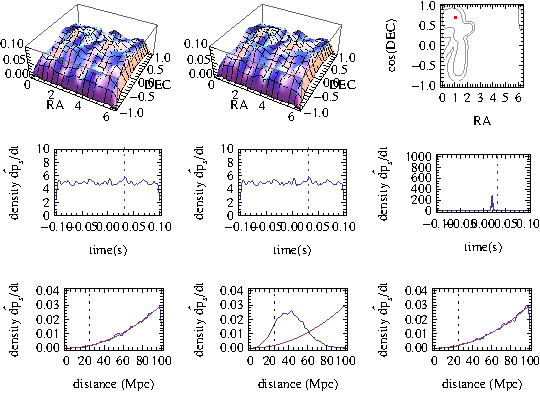
\includegraphics{Figures/fig-mma-DemoSampler.pdf}
\caption{\label{fig:Milestones:DemoSampler:Mathematica}\textbf{Example sampler results (Mathematica)}: Example of a
  uniform sampler (left) and time-of-flight-targeted and distance-targeted sampler (right).  Plots show the sky position distribution (top);
  time distribution (center); and distance distribution (right).   The distance-targeted sampler uses a common distance distribution
}
\end{figure*}
}

\noindent \textbf{Time-of-flight sampler}: Generate random arrival times; convert to a sky position and arrival time.
Examples of these samplers are shown in Figure \ref{fig:Milestones:DemoSampler:Mathematica}.
\begin{itemize}
\item \emph{Inversion tests}: Confirm the low-level time-of-flight code, given time of flights derived from a sky
  location and time, recover that sky location and time.
\item \emph{Sampling distribution}: Plot a sampling distribution in $\hat{n}$ and $t$ derived from a random location. 

 Confirm the location improves (and  converges to the point and mirror point) as the timing errors decrease.
\end{itemize}

\subsection{Milestones and Benchmarks: Sanity check: MCMC extrinsic space (*)}

\noindent \textbf{Why an MCMC  sanity check?}: We want to benchmark our code against a pure MCMC evaluation. Why?  To
find out how many
extra evaluations do we need to fully explore the extrinsic space.  For a single template, to compare the posterior distributions recovered by
our code and another procedure for exploring the extrinsic space.


\editremark{code pending}


\subsection{Milestones and Benchmarks:  Intrinsic exploration (*)}

[Evan's code]

\noindent \textbf{Document prototype exploration procedure}: Trigger values to seed mass range? Fisher matrix?


\noindent \textbf{Basic infrastructure checks}: Confirm we can dump output in the targeted format (e.g., text files) and
generate a dag \editremark{XXX}
\begin{itemize}
\item \emph{Fisher matrix code runs}: The code generates points
\item \emph{Code output}: The code outputs points in the targeted format
\item \emph{DAG generation}: A DAG is generated, including (a) data retrieval; (b) runs

\item \emph{DAG completion}
\end{itemize}




\end{widetext}
\subsection{Requirements}

\noindent \textbf{GraceDB event rate}: Processing time needed for realtime followup is roughly 1/hour.

\noindent \textbf{Operation count}: Fortunately the huge data set is only processed once to generate a \emph{very small}
set of intermediate quantities.  After a few O(N) operations, the \emph{actionable} memory usage is very small.


\noindent \emph{Precompute count}: Typical cores are Gflop.  That means each second of $16kHz$ data (with one flop per
op) requires a few $\mu s$.   
%% Rflop = 7 Giga FLOP/Second 
%% nops = 16384*Ts  FLOP
%% nops/Rflop // SI // N

\noindent \textbf{Memory usage: Computation}: A stupid approach is to use a fixed sampling rate for all time.
%
A 30 min signal at 4kHz with 3 detector REAL8 timeseries $\simeq 180 Mb$.
%% << PhysicalConstants`
%% 30 Minute * 4096/Second * 3 * 8 Byte
%% Convert[%, Mega Byte] // N
Plus, we \textbf{must} create each harmonic tineseries -- with 5 harmonics, this is Gb of storage!  (Plus a factor of few for intermediate
data: the FFTs.)

\noindent \emph{Compressing in time-frequency}: A better approach to the likelihood only evaluates the terms we need.
Memory usage should be \emph{much} more moderate if we only evaluate a handful of inner products. uses (a) tapered sampling rates in
the raw data and template or (b) some intelligent representation (e.g., amplitude-phase representations for the $h_{lm}(f)$).

\noindent \textbf{Memory usage: Output}: 

\noindent \textbf{File I/O} \editremark{don't know} how fast the current disk speeds are, NFS limits, interconnect, etc


\subsection{Routines needed}

\noindent \textbf{Distribution infrastructure}: To evaluate $\int L p$ and $\int p_s L p/p_s$, we first need to define
a distribution object and require certain features:

* request bound on each parameter (e.g., could identify 'light ring normal' and 'light ring width'; 'time
window.geocenter', etc. )

* return random sample from each parameter

* return PDF


\noindent \textbf{Monte carlo integrator}: In terms of $p_s$

* Monte carlo integrator with convergence test (i.e., threshold on $L_{\rm reduced}$ and error tolerance target,
absolute and relative)

** ideally ability to multithread


\noindent \textbf{Ldata and Lsignal}: 



\subsection{Code tests}




\section{Stage 2: Short-term deliverables and selling points (*)} 

\subsection{Results(*)}

\noindent \textbf{Intrinsic mass posterior:}

\noindent \textbf{Reliability of confidence contours}: To demonstrate confidence in each one-dimensional posterior, for
each simulated event $\alpha$ and coordinate $A$ we evaluate the one-dimensional cumulative distribution $P_{\alpha,A}$
and in particular this scalar evaluated at the injection location [$P_{\alpha,A}(x_{\alpha,A})$].  

As an example Figure \ref{fig:ShortTermDemo:OneDCumulativeInjectionRecovery} shows our confidence distribution.
The sources in the sample were drawn randomly from the same prior used \editremark{XXX}

\noindent \textbf{Evidence:}



\begin{figure}
\caption{\textbf{Example of two-dimensional posterior $p(m_1,m_2)$}:
}
\end{figure}

\begin{figure}
\caption{\label{fig:ShortTermDemo:OneDCumulativeInjectionRecovery}\textbf{Example of confidence in confidence
    intervals}: The cumulative distribution of $P_{\alpha,A}(x_{\alpha,A})$ for several variables $A$: chirp mass; mass
  ratio $\eta$; sky location RA; sky location DEC \editremark{do all?}
}
\end{figure}

\subsection{Selling points}

\begin{verbatim}
 -low-latency
 -evidence accurate
 -modular: infrastructure compatible with other uses
\end{verbatim}



\section{Stage N-2: Mid-term deliverables  (*)}
\subsection{Quantity is a quality all its own}
Our speed and performance allow lar

\subsubsection{Revisit prior studies [papers?]}

\noindent \textbf{Fisher matrix breakdown?}: Ilya et al claim the Fisher matrix breaks down for some noise realizations
with moderate SNR.  That's plausible but it'd be nicce to better understand why.  And to be \emph{confident} it's not a
convergence issue.

\subsubsection{New studies}



\section{Stage N-1: Mid-term technical issues (*)}

\noindent \textbf{SNR and breakdowns}: At high SNR, we can \emph{easily} have timing resolution smaller than our
sampling rate (unless using 16 kHz). 

If the SNR is above the low tens, nongaussianities will occur as a matter of course .  [This might in part explain the
  non-Fisher-matrix claims made above.]

\noindent \textbf{PSD sensitivity}: How do we handle the smoothing (1/30 minute  frequency bins?)



\section{Stage N: Long term speculations (*)}


\subsection{Search integration}

\noindent \textbf{As a final coherent stage}: Running with just $(2,\pm 2)$ modes on the triggered masses (exact bank
coincidence) provides a final coherent stage with a confidence statistic (evidence).  Just saying.

If we use exact bank coincidence and a low-dimension $(l,m)$ space, the operations will be sub-minute (few seconds) --
allowing high trigger rates. \editremark{I wonder if this is useful}.

\part{Deprecated notes}

\ForRichardOnly{
\section{Some stuff we are not using}

\subsection{Extrinsic marginalization: Localized sources in $t,\hat{k}$ via time-of-flight }
\label{sec:sub:MarginalizeViaTimeOfFlight}

\noindent \textbf{Arrival-time sampling}: Physical sources will have well-determined arrival times at each detector,
for any significant template.  In our notation, for each detector $k$, each intrinsc parameters $\lambda$, and each
$(l,m)$ there is some pair of real numbers $\rho_{k,lm},t_{k,lm}$  that describes the local maximum's event time and
signal magnitude:
\begin{eqnarray}
\rho_{k,lm} \equiv |Q_{k,lm}(t_{k,lm})|/\sqrt{U_{k,lm,lm}}
\end{eqnarray}
where $Q$ has a local maximum at $t_{k,lm}$.  
[To order of magnitude $\rho_{k,lm}$ is similar to the signal amplitude $\qmstateproduct{\hat{H}_k}{\hat{H}_k}_k$ of the
data in that detector, if a signal is present.]
%
Based on this information, a simple a priori \emph{estimate} for the arrival times $t_1\ldots t_3$ in each detector are possible
[fixing some $(l,m)$ pair -- say (2,2)]: we can build a distribution.

\noindent \emph{Change of variables}: The arrival times are in 1-1 relationship with candidate
event times and sky locations,when physical.  to solve, re-express the arrival times in each detector in terms of the
sky location and geocenter:
\begin{eqnarray}
t_1 = t + \hat{k}\cdot \vec{x}_1 
      = t - \hat{n}(\theta_S,\phi_S)\cdot \vec{x}_1 \\
t_2  = t - \hat{n}(\theta_S,\phi_S)\cdot \vec{x}_2 \\
t_3  = t - \hat{n}(\theta_S,\phi_S)\cdot \vec{x}_3 
\end{eqnarray}
Note in particular that the measure transforms according to
\begin{eqnarray}
 dt_1 dt_2 dt_3  = \sin\theta d\theta d\phi dt (\vec{x}_3-\vec{x}_2)\times(\vec{x}_1-\vec{x}_2)\cdot\hat{n}(\theta,\phi)
\end{eqnarray}
%% coordinate = {t, th, ph};
%% nhat[th_, ph_] := {Sin[th] Cos[ph], Sin[th] Sin[ph], Cos[th]}
%% expr1 = t - {x1, y1, z1}.nhat[th, ph]
%% expr2 = t - {x2, y2, z2}.nhat[th, ph]
%% expr3 = t - {x3, y3, z3}.nhat[th, ph]
%% mydet = Det[{Table[D[expr1, coordinate[[k]]], {k, 1, 3}],
%%     Table[D[expr2, coordinate[[k]]], {k, 1, 3}],
%%     Table[D[expr3, coordinate[[k]]], {k, 1, 3}]}] // FullSimplify
%%  v1 = {x1, y1, z1}
%% v2 = {x2, y2, z2}
%% v3 = {x3, y3, z3}
%% expr = Cross[v3 - v2, v2 - v1].nhat[th, ph] // FullSimplify
%% expr + 1/Sin[th] mydet // Simplify

\begin{shaded}
\noindent \textbf{Inverting these equations in practice: Abstractly}: For each event time we know $\vec{x}_k$ and hence the normal
to the plane of the detectors, $\vec{V}\equiv (\vec{x}_3 -\vec{x}_2)\times(\vec{x}_1-\vec{x}_2)$.  When $\hat{n}\propto
\vec{V}$, then $\hat{n}\cdot (x_1+x_2+x_3)=0$ and hence
\begin{eqnarray}
t = \frac{1}{3}[t_1+t_2+t_3 + \hat{V}\cdot(x_1+x_2+x_3)] 
\end{eqnarray}
The solution for $\hat{n}$ follows by linear algebra, plus scaling to satisfy a constraint:
\begin{eqnarray}
\begin{bmatrix}
\tau_{21} \\ \tau_{31} \\ Z
\end{bmatrix}
=
\begin{bmatrix}
\vec{x}_{21} \\ \vec{x}_{31} \\  \hat{V}
\end{bmatrix}
\begin{bmatrix}
n_x \\ n_y \\ n_z
\end{bmatrix}
\end{eqnarray}
This matrix equation by construction is invertible and tells us the components of $\hat{n}$.  In general they are not
normalized; only discrete choices for $Z$ produce a normalized unit vector $\hat{n}.\hat{n}$; and the quadratic equation
generally has two solutions.

\noindent \textbf{Inverting these equations: Using polar coordinates}: Choose a coordinate system so $x_2-x_1 =|\Delta
r_{21}| \hat{z}$ and so $\hat{x}$ is in the detector plane, forming a right-handed coordinate system.  In this coordinate system we know $\cos \theta = -\Delta r_{21}/(t_2-t_1)$.  The remaining polar angle
must satisfy 
\begin{eqnarray}
\hat{n} = \cos \theta \hat{z} + \hat{x}\sin\theta \cos \phi + \hat{y} \sin\theta \sin\phi \\
\hat{n}\cdot \Delta r_{31} =  \cos \theta \hat{z}.\Delta r_{31} + \sin \theta \cos \phi \hat{x} \cdot \Delta r_{31} \\
\phi = \cos^{-1} - \frac{(t_3-t_1)  - |\Delta r_{31}| \cos \theta_{21}\cos \theta_{31} }{ \sin \theta_{21}  \hat{x}\cdot
  \Delta r_{31}}
\end{eqnarray}

\end{shaded}

\begin{shaded}
\noindent \textbf{Example of distribution: Uncorrelated events?}: One distribution possibility is random times in each detector:
\begin{align}
p_k(t_k) dt_k &= \frac{dt_k}{\sqrt{2\pi  \sigma_t^2/\rho_{k,lm}^2}} \exp - (t_k - t_{k,lm})^2 \rho_{k,lm}^2/2\sigma_t^2 \\
p_1 p_2 p_3 dt_1 dt_2 dt_3 &= \frac{dt_1 dt_2 dt_3 \rho_{1,lm}\rho_{2,lm}\rho_{3,lm}}{(2\pi \sigma_t^2)^{3/2}}
 \exp - \frac{1}{2\sigma_t^2}\left[ (t_1 - t_{1,lm})^2 \rho_{1,lm}^2 + (t_2 - t_{2,lm})^2 \rho_{2,lm}^2 + (t_3 -
   t_{3,lm})^2 \rho_{3,lm}^2 \right]]
\end{align}
Is is trivial to sample normally-distributed  arrival times $t_1,t_2,t_3$ in each detector.  But these can generate
nonphysical possibilities.

\noindent \textbf{Modified distribution: Hard constraints}: A better distribution uses physically-restricted \emph{delay
  time} distributions.  As a concrete example, we know  $\tau_{21}\equiv t_2-t_1$ satisfies $|tau_{12}| \le |r_2
-r_1|/c$ and could draw any delay time for that angle (equivalently, drawing uniformly in the cosine $\hat{n}\cdot
\Delta r_{21}/|\Delta r_{21}$).  For multiple detectors, however, the process of uniform draws introduces an asymmetry:
fixing the first delay time $\tau_{21}$ constrains the physically realizable options for $\tau_{31}$.
\end{shaded}


\noindent \textbf{Lower-dimensional trigonometric sampling}:  The above distributions draw 3d samples in $\hat{n},t$.
After marginalizing over time, the independent-arrival-time model \textbf{implies} a gaussian sky location posterior
\cite{2011CQGra..28j5021F}, of the form [rewriting $\sigma_t/\rho_{1lm} = \sigma_1$ et cetera]
\begin{eqnarray}
p(\hat{n}|t_1,t_2,t_3) \propto \exp(- (\hat{n}-N(t_1,t_2,t_3)).D.(\hat{n}-N(t_1,t_2,t_3))/2)
\end{eqnarray}
[This derivation ignores edge effects.]

\begin{shaded}
The derivation sheds light on the above (and how to generalize our timing solution if the timing errors are unequal).
Let $\bar{t}_k = t_k+\hat{n}\cdot \vec{x}_k$ be the geocentered arrival time derived from $t_k$ and the proposed direction
\begin{eqnarray}
{\cal O}\equiv \Gamma_{kk}(t-\hat{k}\cdot \vec{x}_k -t_k)^2 \equiv \sum_k\Gamma_{kk}(t-\bar{t}_k)^2 
= \bar{\Gamma} t^2 - 2 (\sum_k \Gamma_{kk} \bar{t}_k)t + \sum_k \Gamma_{kk}\bar{t}_k^2 
= \bar{\Gamma}(t-t_*)^2 - \bar{\Gamma} t_*^2  + \sum_k \Gamma_{kk}\bar{t}_k^2 
\end{eqnarray}
When all arrival time errors  \emph{symmetric}, then the time $t$ which maximizes the likelihood is  independent of the
sky location $\hat{n}$; in general, however, the optimal time $t_*$ is
\begin{eqnarray}
t_*  = (\sum_k \Gamma_{kk} \bar{t}_k)/\sum_k \Gamma_{kk} \equiv \left<\bar{t}\right>
\end{eqnarray}
where I use a suitable ``average'' notation to weight over interferometers. 
Completing the square leads to a marginalized quadratic (after integrating out other variables)
\begin{eqnarray}
{\cal O}_{\rm marg}\equiv - \bar{\Gamma} t_*^2  + \sum_k \Gamma_{kk}\bar{t}_k^2  
 = \bar{\Gamma}\left[ -\left<\bar{t}\right>^2 + \left<\bar{t}^2 \right> \right]
 = \bar{\Gamma}\left[ -\left<t_{\rm measured}+\hat{n}\vec{x}\right>^2 + \left<(t_{\rm measured}+\hat{n}\vec{x})^2
  \right>
 \right]
\end{eqnarray}
Now reorganize the expression to group terms quadratic and linear in $\hat{n}$ to identify the best-fit sky position, et
cetera:
\begin{eqnarray}
{\cal O}_{\rm marg} \equiv 
{\color{blue}\bar{\Gamma}n_a n_b \left[
   -\left<\vec{x}_a\right>\left<\vec{x}_b\right> + \left<\vec{x}_a \vec{x}_b\right>
 \right]
}
+{ 2 \bar{\Gamma}n_a  \left[
   -\left<\vec{x}_a \right>\left<t_{\rm measured}\right> + \left< t_{\rm measured} \vec{x}_b\right>
 \right]
}
+  \bar{\Gamma}  \left[
 -\left<t_{\rm measured}\right>^2 + \left<(t_{\rm measured})^2 \right>
 \right]
\end{eqnarray}
The first  term (blue) tell us the shape of the sky position posterior on the plane of the sky.  The second term
(combined with the first) tells us the best-fitting sky position
\end{shaded}
} % End hide


\subsection{Extrinsic marginalization: Distance }

\noindent \textbf{``Physical'' distance distribution}: The distance prior is dominated by the largest distances allowed.  Conversely,
the distance posterior is of order unity.
%
For any \emph{individual} sky location, inclination,  and template, the actual distance posterior has the form [Eq. \ref{eq:ComputeRhoViaInnerProductMatrix}]editremark{See eqna}
\begin{eqnarray}
p(r)dr \propto  r^2 dr \exp \left[ -\rho_{\rm ref}^2 (d_{\rm ref}/d)^2//2 + \qmstateproduct{{\cal S}(\hat{n})}{h_{\rm
      ref}}_{\rm ref} (d_{\rm
    ref}/d) \right]
\end{eqnarray}
where ${\cal S}(\hat{n})$ is a sky-position-dependent resumming of the data into quasi-coherent form; where
$\qmstateproduct{.}{.}_{\rm ref}$ refers to the weighted inner product described near
Eq. (\ref{eq:def:GeocenteredInnerProductWithData}); and where $h_{\rm ref}$ and $\rho_{\rm ref}$ refer to the signal
and signal amplitude at the proposed model parameters, evaluated at $d=d_{\rm ref}$.  
%

For any specific source orientation and sky location, the physical distance distribution is extremely narrow.
Marginalizing over orientations, the distance distribution becomes broad.  By implication, if the
same sampling distribution must be used for all orientations, the sampling distribution must \emph{also} be broad.  So
we can't use this.


\begin{shaded}
\noindent \textbf{Distance targeting with trigger [tempate-dependent sampling]}:  One proposal is a form like this
So in practice the distance distribution has the form
\begin{eqnarray}
p(r)dr \propto r^2 dr \exp[ (-(r_0/r)^2/2 + (r_o/r)){\cal A}]
\end{eqnarray}
for some constants $r_o$ and ${\cal A}$ to be provided \editremark{provide a specific formula}.  An example of distance-targeted sampling is shown in Figure
\ref{fig:Milestones:DemoSampler:Mathematica}.  

Is this useful?  \textbf{Is is not a very useful form}:
\begin{itemize}
\item  if the amplitude is large (=comparable to expected) this procedure sets an EXTREMELY tight prior on the signal amplitude, but
only a loose prior on the distance (=because of inclination degeneracy)

\item this kind of prior sets a natural \emph{lower} limit, but not a strong upper one: as $r \rightarrow \infty$, the
  exponential approaches a constant
\end{itemize}

We can modify this expression to use a 

\noindent \textbf{Distance targeting with template [tempate-dependent sampling]}: We are free to \emph{use a different
  sampling distribution at each template.}  Suppose we have a candidate template.  Putting that source at a
reference distance ($d_{\rm ref}=100 Mpc$) in any one detector tells us the distance posterior for that template \emph{automatically}: we
are free to use that posterior as a sampling distribution.   \editremark{write down}
\end{shaded}


\noindent \textbf{Ad hoc distance distributions}: Suppose we can place a confident upper bound on the source distance (e.g.,
from the peak amplitude).  A good sampling distribution covers the whole range, with plausible behavior at small
distances.
%
I don't see a good reason to use a tightly peaked sampling prior, except to exclude zero; options include  uniform over
that range; volumetric with cutoff; or something else (e.g., a parabola over that range).



\noindent \textbf{Data-dependent distance distributions}: We are free to use any sampling distribution to evaluate the
integral, including a data-dependent one.   A signal with a strong peak in $\qmstateproduct{\hat{H}}{h}$ -- equvalently,
in the $Q_{k,lm}$ -- must be close by.  Precisely how close depends on the orientation source orientation; however, we
can confidently place an upper bound, using an optimally oriented source (derived independently from each IFO).

So,  reconstruct the optimally oriented distance using Eq. (\ref{eq:SpecialCase:SingleIFOOptimalOrientation}), a model for the distance to an
optimally oriented source overhead a single detector:
\begin{eqnarray}
\bar{Q}_k \equiv  \text{max}_t |Q_{k,22}| \simeq \frac{d_{\rm ref}}{2 d} \sqrt{\frac{5}{4\pi}} U_{k,22,22} \\
\hat{d} \equiv \frac{1}{n_{det}}\sum_k\frac{U_{k,22,22}}{\bar{Q}_k} \frac{d_{\rm ref}}{2} \sqrt{\frac{5}{4\pi}}
\end{eqnarray}
Not the best estimate...so we should pad it with a lorentzian. \editremark{implement}

\end{widetext}


\part{Richard's notes to self}


* NOW IT IS EASY to truncate the number of fitting points to a small time window: after rolling, take a small subset

* SUGGESTION FOR DATA GENERATION: slow because we completely regenerate the whole signal 3 times, rather than
  project the same signal onto each IFO

\section{Design philosophy}

Software development research and my experience suggests data fuzzing and persistnt unit tests are a much better way to
identify and prevent bugs than code/patch review.  Code and patch review, like congress, allows only incremental
improvement to an existing codebase.  It just doesn't find bugs.  

A ``clean'' code (=only having ``used'' routines), supported by documented ``investigations'', works best under
extremely controlled circumstances -- for example, modular code with deliverables, where the inputs, outputs, and
approximations needed are set up and thoroughly documented.  The code structure needs to be frozen at design stage.  
And it's extremely difficult to unit test changes without multiple copies of the codebase.

Before distilling to a ``clean'' code, a \textbf{development} code (``hackathon mode'') can identify approximations and
choices, document and validate deliverables with unit tests.  Unit tests, if well written, are excellent documentation.

The challenge from going to a development branch to a ``clean'' branch is distillation -- you need to make sure that
doesn't introduce errors when code is eliminated and ``simplified''.

Finally, patches as a method of communication.  On a large-scale project, patch review is only as good as the people
involved, and requires perfect dilligence.  People don't function that way.  So patch review is a nice reporting tool
for management and nominal Q/A, to guarantee people are well-behaved (e.g., like TERs)...but doesn't by itself
provide any added value to code quality or correctness.
  A better method is embedded tests.
\begin{verbatim}
PRINCIPLES: Development
     - rapid prototyping to develop design
     - identify routines, with unit tests. Unit tests provide documentation, validation, and debugging aid
	- quasi-realistic 'unit tests' are built into the many test_* functions.
	- not a pedant: life is short
     - prefer strongly controlled circumstances for the unit tests, not end-to-end, to isolate features. 
\end{verbatim}

\subsection{Assorted rants}

\noindent \textbf{For loops}: For loops with human-entered limits produce (fencepost) errors \textbf{very} frequently.
These errors are among the most difficult to identify through code review. 
Any sane programmer uses language or library features (e.g., map; iterators; etc) to avoid manual iteration.  In
numerical code, these features often come with added benefits (e.g., parallelization and/or vectorization under the hood).  
\textbf{Don't use for loops. Just don't.} Let computers do what they're good at (perfect dilligence, attention to
detail) and humans do what they're good at (design).

\section{Python implementation}

\noindent \textbf{Input check}: 

* Fourier convention: $\tilde{h}_{22}$ should have only positive frequencies \editremark{checkme}

\noindent \textbf{Timeshifts?}: Still not fixed. But at least we are coherent.


\noindent \textbf{Operations check}

* make sure frequencies are consistently set EVERYWHERE.  It's very important to get all the PSD integrals using a
consistent lower frequency! \editremark{FIX ME}

\noindent \textbf{Intermediate structures}



* $Q$ timeseries has broad support

* \textbf{Distance scaling} incorrectx

\section{Mathematica implementation}

\noindent \textbf{Mathematica memory usage}: Huge overhead for arrays.  Calibrate usage for frame files and control
memory bloat

\noindent \textbf{Triangulation sampler}: Implement!

\noindent \textbf{Mass-dependent data length?}: Change data length depending on trigger chirp mass to reduce computation time.


\noindent \textbf{Converter}: Dump to quasi-MCMC output (\texttt{BayesianInport})

\section{Python implementaiton}



\subsection{Remaining bugs}
\noindent \textbf{Sign vs Pankow injection}: Phase difference, it seeems



\subsection{Implementation issues to remember}



\noindent \textbf{Python swig time }: Be careful re the automagic time conversion. It is \textbf{very important} to make
sure all time quantities remain GPSTime objects...and very easy to slip up when passing arguments and throw a float
instead.  
\begin{shaded}
\begin{verbatim}
from factored_likelihood import *
detector = lalsim.DetectorPrefixToLALDetector('H1')
 tArrive = ComputeArrivalTimeAtDetector("H1", 0,0,0)   # this is not a GPStime
tArriveB = ComputeArrivalTimeAtDetector("H1",0,0,lal.GPSTimeNow())   # this is a GPS time
\end{verbatim}
\end{shaded}

\noindent \textbf{Reference phase}: Be careful to adopt it consistently

\subsection{Tests to implement}
\noindent \textbf{Serial pipeline}: Rather than parallelize across the cluster, do a full zero-spin serial operation.
It will be easier to document the physics and infrastructure if it's in one code.

Make $L_{\rm marg}(m_1,m_2)$, recovery $p-p$ plots, etc

\noindent \textbf{Serial sky localization code}: Test our comparison against Bayesstar

\noindent \textbf{Mass-dependent data length?}: Change data length depending on trigger chirp mass to reduce computation time.


\subsection{Python MPI and parallelization}

\noindent \textbf{PythonMPI}: Apparently python MPI and even python multithreading is possible with cython (=compiling an extension, and releasing the
global interpreter lock).  So we \textbf{ought} to be able to capture all the advantages we're looking for.
\begin{verbatim}
http://mpi4py.scipy.org/docs/usrman/tutorial.html  # mpi
http://www.vallis.org/salon/summary-8.html         # openmp
http://archive.euroscipy.org/talk/6857
\end{verbatim}

\noindent \textbf{Faster low-level calls: typing, cython, ...}: Should be massive speed improvement.  Type checking on
our nested loops causes enormous problems -- the code is just too slow.
\begin{verbatim}
http://numba.pydata.org/numba-doc/0.11/types.html
http://jakevdp.github.io/blog/2013/06/15/numba-vs-cython-take-2/
http://www.slideshare.net/teoliphant/numba-siam-2013
\end{verbatim}
%http://stackoverflow.com/questions/8097408/why-python-is-so-slow-for-a-simple-loop

\noindent \textbf{Multiprocessing}:  A hack to achieve mildly better flow
\begin{verbatim}
http://docs.python.org/dev/library/threading.html#	
http://docs.python.org/dev/library/multiprocessing.html
http://stackoverflow.com/questions/2846653/python-multithreading-for-dummies
\end{verbatim}

\subsection{Pipeline generation (*)}


\appendix



\section{Gravy issues: Things to think about but not critical now}

% http://www.physics.gla.ac.uk/igr/GWbursts2012/pages/program/slides/MondayPM/Favata.pdf
\emph{Physics check 1: Memory modes}: The $m=0$ memory modes \cite{2009PhRvD..80b4002F,2009ApJ...696L.159F,2010CQGra..27h4036F,2011PhRvD..84l4013F} aren't consistently implemented: present with
  TaylorTN but \emph{not} with SpinTaylorT4.   If they \emph{are}
  implemented, their spectrum is \textbf{incredibly sensitive to numerical effects: start and particularly the abrupt
    end of the signal}.  Finally, memory is \textbf{physically incompatible with zero padding}: we need to ``pad and
  extend'', not zero pad!    But for non-IMR waveforms, we don't know how to do that without \textbf{explicitly} knowing
  which parts of the signal are memory!

Do you care?  Memory modes are \emph{not} always sufficiently insignificant: if the signal is short and the number of cycles
$N_{c}$ is small compared to $1/\rho^2$, then these overlaps matter:
\begin{eqnarray}
\qmstateproduct{h_{22}}{h_{20}} \simeq O(1) \times \qmstateproduct{h_{22}}{h_{22}}/N_c 
\end{eqnarray}
You should confirm these overlaps are \emph{not} zero with \texttt{TaylorT4} but \emph{are} zero for
\texttt{SpinTaylorT4} (when implemented).

\textbf{Should we fix it now?} No.  It's a relatively minor fix; everyone made this mistake; it's less important for
long aLIGO waveforms. \editremark{Gravy item for the paper}

\textbf{Should we manually set m=0 modes to zero for nonprecessing?}: Not yet...

\begin{shaded}
\noindent \textbf{Gravitational wave memory}: One informal   ad-hoc argument suggesting significant memory ($\tilde{h}(f)\propto f^{-1}$)
  relies on $h$ changing by a nonzero amount in the $(l,0)$ modes.    These discontinuities are inevitable consequences
  of radiation and insure $\tilde{h}$ decays as $1/f$ at high frequency.

\noindent \textbf{Do we implement it?}: Nope.  And what we do implement is seriously broken

\noindent \textbf{How can we fix it?}

\noindent \textbf{What are the physical consequences of memory modes?}: The memory modes have nonzero overlap with
everything. [For a nonprecessing binary, $\tilde{h}^{\rm mem} \simeq i \Delta h/2\pi f$ below a characteristic cutoff
scale (i.e., the merger timescale).]
\end{shaded}
\section{Notation issues: Comparing with standard notation}

\subsection{Signal amplitude}

\noindent \textbf{Single-interferometer: Complex notation}
For a single perpendicular-arm detector with waves \emph{propagating from} $\hat{n}=n(\theta,\phi)$ on the sky and with
polarization angle $\psi$ \emph{along that direction} \editremark{check signs}
\begin{subequations}
\label{eq:SingleIFOResponse}
\begin{eqnarray}
\begin{bmatrix}
F_+ \\ F_\times 
\end{bmatrix}
&=& \begin{bmatrix}
e_+(z):e_+^{(gw)}(-\hat{n},\psi) \\
e_+:e_\times^{(gw)} 
\end{bmatrix}
 \\
&=& 
\begin{bmatrix}
\cos 2\psi & \sin 2 \psi \\
- \sin 2 \psi & \cos 2 \psi
\end{bmatrix}
\begin{bmatrix}
\frac{1}{2} (1+\cos^2\theta) \cos2\phi  \\
\cos \theta \sin 2 \phi
\end{bmatrix} \nonumber
\\
F_\mathrm{+} &=&
 \frac{1}{2}(1+\cos^{2} \theta) \cos 2 \phi \cos 2 \psi
\nonumber\\ &+& \cos \theta \sin 2 \phi \sin 2 \psi \, \\ 
F_\mathrm{\times} &=&- \frac{1}{2}(1+\cos^{2} \theta) \sin 2 \phi \cos 2 \psi
\nonumber \\ &+& \cos \theta \cos 2 \phi \sin 2 \psi
\end{eqnarray}
\end{subequations}
where $e_+^{(gw)}$ are the appropriately rotation-modified structures
previously and $\psi$ is a polarization orientation (i.e., the third
euler angle associated with the rotation operator; see the SU(2) reference).  
%
In the text it will be helpful to express them in complex form:
\begin{eqnarray}
{} [F_{+}+i F_{\times}](\hat{n},\psi) &=& \frac{\sqrt{4\pi}}{\sqrt{5}}\left[ e^{-2i\psi}\Y{-2}_{22} +
  e^{+2i\psi}\Y{-2}_{2,-2}  \right] 
\end{eqnarray}


\noindent \textbf{Conventional signal amplitude expression}: 
A nonprecessing source dominated by a single pair of conjugate $(2,\pm 2)$ modes has a simple signal and a well-known
signal-to-noise ratio expression.  That standard expression (replacing $\iota \rightarrow \theta_E$ and $\phi_c \rightarrow \phi_E$) has the
following form \editremark{signs certainly wrong}
\begin{subequations}
\label{eq:SingleIFO:AmplitudeSquared}
\begin{align}
H_1 &= F_+(\theta_S,\phi_s,0) h_+ + F_\times(\theta_S,\phi_S,0)h_\times \\
    &= \text{Re} (F_++i F_\times) e^{-2i\psi} [\frac{1+\cos \theta^2_E}{2}h_{+,\hat{z}} - i \cos \theta_S
  h_{\times,\hat{z}}] \\
 &= {\cal F}_+ h_{+,\hat{z}} + {\cal F}_{\times} h_{\times, \hat{z}} \\
{\cal F}_+ &= F_+(\theta_S,\phi_S,\psi)\frac{ 1+\cos^2 \theta_E}{2} + F_\times(\theta_S,\phi_S,\psi) \cos \theta_E \\
{\cal F}_\times &= F_\times(\theta_S,\phi_S,\psi) \cos \theta_E  + F_+(\theta_S,\phi_S,\psi)\frac{1+\cos^2\theta}{2}\\
\end{align}
where we absorb inclination and polarization dependence into the generalized detector response functions ${\cal F}$.
Substituting into the signal amplitude expression and using orthogonality and equal amplitude of $h_{+,\hat{z}}$ and $h_{\times, \hat{z}}$:
\begin{align}
\qmstateproduct{H_1}{H_1}_1 
  &= \qmstateproduct{h_{+,z}}{h_+,z} [{\cal F}_+^2  + {\cal F}_\times^2]
% \text{Re}[(F_++i F_\times) e^{-2i\psi} \frac{1+\cos^2 \theta_E}{2}]^2 \nonumber \\ & 
%+  \text{Im}[(F_++i F_\times) e^{-2i\psi} \cos \theta_E]^2
\end{align}
\end{subequations}

\section{Extensions and comparison: F statistic}

In GW searches,  polarization phase marginalization can be done simultaneously.  At each timesample, we expected we could
 marginalize \emph{analytically} over polarization phase, with a bessel function. 


\subsection{Marginalizing in the polarization angle}

\begin{shaded}
\noindent \textbf{Template amplitude}: Using the $\sigma,\epsilon$ notation of \citet{CutlerFlanagan:1994}, the signal amplitude term has the form $\rho^2 = \sigma
\rho_0^2(1+\epsilon \cos 4(\psi-\psi_0))$ where $\rho_0^2$ is the amplitude of a source directly overhead a single
detector and $\sigma,\epsilon$ are derived from the beampattern functions:
\begin{eqnarray}
C_{\lambda \lambda'}&=& \sum_k \begin{bmatrix}
F_+^2 & F_+F_\times \\
F_\times F_+ & F_\times^2
\end{bmatrix}\\
&=& \sum_k [P_k : \hat{e}_\lambda(\hat{n})] [P_k : \hat{e}_{\lambda'}(\hat{n})]  \nonumber \\
& =& \sigma U\begin{bmatrix} (1+\epsilon) & 0 \\ 0 & 1-\epsilon \end{bmatrix} U^{-1} 
\end{eqnarray}
where $U$ is a unitary transformation that diagonalizes $C$.

\noindent \textbf{Response against data}: By contrast, for a fixed data set, the second term in the likelihood
necessarily transforms like $h$: purely sinusoidally in polarization angle
\begin{eqnarray}
\rho \hat{\rho} = A \cos 2\psi + B \cos 2 \psi
\end{eqnarray}
\noindent \textbf{Marginalizing?}: If this were the only term in the likelihood -- for example, for an isotropic network
--  we could marginalize exactly: \textbf{BUT THIS IS NOT TRUE}
\begin{align}
\ln L  &= [\ln L]_c \cos 2\psi + [\ln L]_s \sin 2\psi = \ln L_0 \cos 2(\psi-\psi_0)  \\
\ln L_0 &= \sqrt{[\ln L]_c^2+[\ln L]_c^2} \\
\int_0^{\pi}\frac{ d\psi}{\pi} L &= \frac{1}{\pi}I_0(\ln L_0)
\end{align}
In general $\rho$ depends on $\psi$, so we can't: both $\cos 2\phi$ and $\cos 4\psi$ appear in the exponential, unless
the network has $\epsilon=0$ (i.e., equal sensitivity to both polarizations).
\end{shaded}



\subsection{F statistic}

When viewed as maximization, this approach resembles the F statistic
\cite{1998PhRvD..58f3001J,2005PhRvD..72f3006C,2012PhRvD..86l3010K,gwastro-HarryFairhurst-CoherentTargetedSearch}\cite{BCV:PTF}.



\noindent \textbf{F statistic versus our approach}: The F statistic approach uses 4 real basis functions (2 polarizations
plus cosine, sine chirp in each).  Including distance, these 4 basis functions have arbitrary coefficients in each
signal: all possible realizations exist and correspond to different physical configurations with different
$(d,\theta_S,\phi_S,\psi)$.  Maximization (or marginalization) of the likelihood over these four amplitudes is possible
analytically! Why? Because the likelihood  $-\rho^2/2 + \ln L_{\rm data}$ has the form \editremark{roughly speaking}
\begin{eqnarray}
\ln L \propto a_\alpha \sum_k\qmstateproduct{h_\alpha}{\hat{H}_k}_k + a_\alpha a_\beta \qmstateproduct{h_{\alpha}}{h_\beta}_k
\end{eqnarray}
which, modulo measure factors, can be marginalized via gaussian integral tricks.

In our approach,  more than 4 real basis functions exist.  Their amplitudes are \textbf{not independent}, because there
are more than 4 of them (but still only 4 real-valued parameters). 

Additionally, in our approach, \textbf{the sine and cosine chirp are not exactly orthgonal, and we have memory modes}
(in general).  This effect is noticable in iLIGO-scale (short) signals

 The F-statistic trick is a possible \emph{approximation} but not valid in general, particularly  not  for precessing binaries

\clearpage
\section{Marginalizing over Distance}
Following the earlier notation, the total likelihood can be written as 
\begin{eqnarray}
\ln L &&\equiv \ln L_{\rm model} + \ln L_{\rm data} \\
\ln L_{\rm model} &&\equiv -\frac{1}{2} \frac{1}{r^2} \sum_k \qmstateproduct{H_k}{H_k}_k = - \frac{1}{2} \frac{\sigma^2}{r^2} \\
\ln L_{\rm data} &&\equiv  \frac{1}{r} \sum_k \qmstateproduct{H_k}{\hat{H}_k}_k = \frac{z}{r} \; .
\end{eqnarray}
Here, the factors of distance have been explicitly pulled out and the waveform
$H_k$ is to be normalized to a canonical distance (e.g. 100Mpc as used
earlier). 

The traditional signal-to-noise ratio is defined as $\rho = z / \sigma$. In the
presence of zero-mean noise, uncorrelated between detectors, and in the absence
of a signal, this is a Gaussian random variable with zero mean and unit
variance. If a signal $H_k/r$ is present in the data, the mean $\overline{\rho}
= \sigma /r$ where the distance is in canonical distance units. This leads to
an alternate interpretation of $\sigma$ as the distance to a binary that gives
$\overline{\rho}=1$. 

The distance prior is uniform in volume out to some distance $r_{\mathrm{max}}$
which should be big enough not to artificially cut off the posterior, but small
enough not to require a correct treatment of cosmology. With this notation, the
marginalization reduces to computing the the integral
\begin{equation}
I = \int_0^{r_{\mathrm{max}}} r^2 \exp\left[ \frac{z}{r} - \frac{\sigma^2}{2 r^2} \right] dr \; .
\end{equation}
It is also worth noting that typically we obtain an array of values $z(t)$
corresponding to different geocentric times for the signal. We already make use
of this to speed up the marginalization over time. This will be important when
it comes to implementation. On the other hand, the intrinsic parameters are fixed as are $\iota$, $\alpha$, $\delta$, $\Phi$, and $\psi$. Usually, we also fix the distance $r$, the point of this section is to use the simple scaling in distance to allow us to carry out the marginalization over distance and the marginalization over time without having to make more draws. 

The deceptively simple looking integral over $r$ cannot be solved in terms of
known (special) functions and so we are left with approximations or numerical
integration schemes. To this end, it is convenient to use the following quantities
\begin{eqnarray}
y &=& \frac{r_{\mathrm{max}}}{r} \\
\sigmahat &=& \frac{\sigma}{r_{\mathrm{max}}} \; .
\end{eqnarray}
Notice that $\sigmahat$ depends both on the sensitivity of the instrument and
the upper bound on $r$ used in the integral. Moreover, if $r_{\mathrm{max}}$ is
chosen to be at least 16 times the largest horizon distance for any binary under 
consideration, then
\begin{equation}
0 \leq \sigmahat \leq 0.5 \; .
\end{equation}
This constraint on $\sigmahat$ simplifies the process of finding an
approximation to the integral. In terms of these new variables, the integral is
\begin{eqnarray}
I &=& r_{\mathrm{max}}^3 \int_1^\infty y^{-4} \exp\left[ \rho \sigmahat y - \sigmahat^2 y^2 / 2 \right] dy \\
  &=&r_{\mathrm{max}}^3 e^{\rho^2/2} \int_1^\infty y^{-4} e^{- (y - \rho / \sigmahat)^2 / 2} dy 
    \label{eq:distmarg}
\end{eqnarray}
We note the integrand has extrema at
\begin{equation}
y_\pm = \frac{\rho}{2 \sigmahat} \left[ 1 \pm \sqrt{ 1 - 16 / \rho^2 } \right]
\end{equation}
and hence there are no extrema for $\rho < 4$. There are a number of useful
approximations and limits which can help to understand the behavior of this
integral.

Consider first the limit $\rho \rightarrow \infty$ for fixed $\sigmahat$, one
can approximate the integral as
\begin{eqnarray}
I &\approx& r_{\mathrm{max}}^3 e^{\rho^2/2} \int_1^\infty (\rho/\sigmahat)^{-4} e^{- (y - \rho / \sigmahat)^2 / 2} dy \\
I^+ &=&\frac{ r_{\mathrm{max}}^3 \sigmahat^3 e^{\rho^2/2} }{ \rho^4 } \sqrt{\frac{\pi}{2}} \left[ 1 + \epsilon \erf ( \epsilon (\rho -a)/\sqrt{2} ) \right] \label{eq:largerho}
\end{eqnarray}
where $\epsilon = \sgn(rho-a)$. This gives the expected large signal to noise
scaling with a predicted factor in front of the exponential. 

The next interesting limit is $\sigmahat \rightarrow 0$ keeping everything else
fixed. The result is easily confirmed to be 
\begin{equation}
\lim_{\sigmahat \rightarrow 0} I \rightarrow \frac{ r_{\mathrm{max}}^3 }{ 3 } \; . \label{eq:sigmazero}
\end{equation}

Finally, consider the regime where $\rho \ll \sigmahat$ in which the integral
is dominated by contributions coming from near $y=1$. Expanding $\exp[(y - \rho
/ \sigmahat)^2 / 2]$ about $y=1$ and subsituting it into the right hand side of
(\ref{eq:distmarg}), we find 
\begin{equation} 
I^- = \frac{r_{\mathrm{max}}^3 }{ 3 } \exp[\rho \sigmahat - \sigmahat^2/2] \; . \label{eq:smallrho}
\end{equation}
Naturally, this reduces to (\ref{eq:sigmazero}) as $\sigmahat \rightarrow 0$. 

It is now easy to write an approximation to $I$ that could be used in our code
to approximate the integral over distance as
\begin{equation} 
I = I^- + \Theta(\rho - 2) I^+ \; .
\end{equation}
The step-function at $\rho=2$ is needed to avoid divergences in $I^+$ at $\rho=0$. 

\begin{figure}
\includegraphics[width=0.5\textwidth]{Figures/i-v-rho}
\caption{\label{fig:distmarg}
The marginalized integral $I$ as a function of the signal-to-noise ratio $\rho$
for various $\sigmahat$. The solid lines are the numerical integration and the
circles represent the approximation. There is excellent visual agreement.}
\end{figure}

\begin{figure}
\includegraphics[width=0.5\textwidth]{Figures/i-error-v-i}
\caption{\label{fig:distmarg}
The ratio of the numerical value to the approximation of the marginalized
integral $I$ as a function of the signal-to-noise ratio $\rho$ for various
$\sigmahat$. Clearly the approximation breaks down for small $\rho$ as
$\sigmahat$ increases. Nevertheless, the approximation is still reasonably good
for a broad range of $\rho$ and $\sigmahat$ values. }
\end{figure}










\bibliography{overviewexport}
\end{document}

